%  LaTeX support: latex@mdpi.com 
%  For support, please attach all files needed for compiling as well as the log file, and specify your operating system, LaTeX version, and LaTeX editor.

%=================================================================
\documentclass[mathematics,article,accept,pdftex,moreauthors]{Definitions/mdpi} 
% For posting an early version of this manuscript as a preprint, you may use "preprints" as the journal and change "submit" to "accept". The document class line would be, e.g., \documentclass[preprints,article,accept,moreauthors,pdftex]{mdpi}. This is especially recommended for submission to arXiv, where line numbers should be removed before posting. For preprints.org, the editorial staff will make this change immediately prior to posting.

%--------------------
% Class Options:
%--------------------
%----------
% journal
%----------
% Choose between the following MDPI journals:
% acoustics, actuators, addictions, admsci, adolescents, aerospace, agriculture, agriengineering, agronomy, ai, algorithms, allergies, alloys, analytica, animals, antibiotics, antibodies, antioxidants, applbiosci, appliedchem, appliedmath, applmech, applmicrobiol, applnano, applsci, aquacj, architecture, arts, asc, asi, astronomy, atmosphere, atoms, audiolres, automation, axioms, bacteria, batteries, bdcc, behavsci, beverages, biochem, bioengineering, biologics, biology, biomass, biomechanics, biomed, biomedicines, biomedinformatics, biomimetics, biomolecules, biophysica, biosensors, biotech, birds, bloods, blsf, brainsci, breath, buildings, businesses, cancers, carbon, cardiogenetics, catalysts, cells, ceramics, challenges, chemengineering, chemistry, chemosensors, chemproc, children, chips, cimb, civileng, cleantechnol, climate, clinpract, clockssleep, cmd, coasts, coatings, colloids, colorants, commodities, compounds, computation, computers, condensedmatter, conservation, constrmater, cosmetics, covid, crops, cryptography, crystals, csmf, ctn, curroncol, currophthalmol, cyber, dairy, data, dentistry, dermato, dermatopathology, designs, diabetology, diagnostics, dietetics, digital, disabilities, diseases, diversity, dna, drones, dynamics, earth, ebj, ecologies, econometrics, economies, education, ejihpe, electricity, electrochem, electronicmat, electronics, encyclopedia, endocrines, energies, eng, engproc, ent, entomology, entropy, environments, environsciproc, epidemiologia, epigenomes, est, fermentation, fibers, fintech, fire, fishes, fluids, foods, forecasting, forensicsci, forests, foundations, fractalfract, fuels, futureinternet, futureparasites, futurepharmacol, futurephys, futuretransp, galaxies, games, gases, gastroent, gastrointestdisord, gels, genealogy, genes, geographies, geohazards, geomatics, geosciences, geotechnics, geriatrics, hazardousmatters, healthcare, hearts, hemato, heritage, highthroughput, histories, horticulturae, humanities, humans, hydrobiology, hydrogen, hydrology, hygiene, idr, ijerph, ijfs, ijgi, ijms, ijns, ijtm, ijtpp, immuno, informatics, information, infrastructures, inorganics, insects, instruments, inventions, iot, j, jal, jcdd, jcm, jcp, jcs, jdb, jeta, jfb, jfmk, jimaging, jintelligence, jlpea, jmmp, jmp, jmse, jne, jnt, jof, joitmc, jor, journalmedia, jox, jpm, jrfm, jsan, jtaer, jzbg, kidney, kidneydial, knowledge, land, languages, laws, life, liquids, literature, livers, logics, logistics, lubricants, lymphatics, machines, macromol, magnetism, magnetochemistry, make, marinedrugs, materials, materproc, mathematics, mca, measurements, medicina, medicines, medsci, membranes, merits, metabolites, metals, meteorology, methane, metrology, micro, microarrays, microbiolres, micromachines, microorganisms, microplastics, minerals, mining, modelling, molbank, molecules, mps, msf, mti, muscles, nanoenergyadv, nanomanufacturing, nanomaterials, ncrna, network, neuroglia, neurolint, neurosci, nitrogen, notspecified, nri, nursrep, nutraceuticals, nutrients, obesities, oceans, ohbm, onco, oncopathology, optics, oral, organics, organoids, osteology, oxygen, parasites, parasitologia, particles, pathogens, pathophysiology, pediatrrep, pharmaceuticals, pharmaceutics, pharmacoepidemiology, pharmacy, philosophies, photochem, photonics, phycology, physchem, physics, physiologia, plants, plasma, pollutants, polymers, polysaccharides, poultry, powders, preprints, proceedings, processes, prosthesis, proteomes, psf, psych, psychiatryint, psychoactives, publications, quantumrep, quaternary, qubs, radiation, reactions, recycling, regeneration, religions, remotesensing, reports, reprodmed, resources, rheumato, risks, robotics, ruminants, safety, sci, scipharm, seeds, sensors, separations, sexes, signals, sinusitis, skins, smartcities, sna, societies, socsci, software, soilsystems, solar, solids, sports, standards, stats, stresses, surfaces, surgeries, suschem, sustainability, symmetry, synbio, systems, taxonomy, technologies, telecom, test, textiles, thalassrep, thermo, tomography, tourismhosp, toxics, toxins, transplantology, transportation, traumacare, traumas, tropicalmed, universe, urbansci, uro, vaccines, vehicles, venereology, vetsci, vibration, viruses, vision, waste, water, wem, wevj, wind, women, world, youth, zoonoticdis 

%---------
% article
%---------
% The default type of manuscript is "article", but can be replaced by: 
% abstract, addendum, article, book, bookreview, briefreport, casereport, comment, commentary, communication, conferenceproceedings, correction, conferencereport, entry, expressionofconcern, extendedabstract, datadescriptor, editorial, essay, erratum, hypothesis, interestingimage, obituary, opinion, projectreport, reply, retraction, review, perspective, protocol, shortnote, studyprotocol, systematicreview, supfile, technicalnote, viewpoint, guidelines, registeredreport, tutorial
% supfile = supplementary materials

%----------
% submit
%----------
% The class option "submit" will be changed to "accept" by the Editorial Office when the paper is accepted. This will only make changes to the frontpage (e.g., the logo of the journal will get visible), the headings, and the copyright information. Also, line numbering will be removed. Journal info and pagination for accepted papers will also be assigned by the Editorial Office.

%------------------
% moreauthors
%------------------
% If there is only one author the class option oneauthor should be used. Otherwise use the class option moreauthors.

%---------
% pdftex
%---------
% The option pdftex is for use with pdfLaTeX. If eps figures are used, remove the option pdftex and use LaTeX and dvi2pdf.

%=================================================================
% MDPI internal commands
\firstpage{1} 
\makeatletter 
\setcounter{page}{\@firstpage} 
\makeatother
\pubvolume{1}
\issuenum{1}
\articlenumber{0}
\pubyear{2022}
\copyrightyear{2022}
\externaleditor{{Academic Editors: Theodore E. Simos and Charampos Tsitouras}} 
\datereceived{6 July 2022} 
%\daterevised{} % Only for the journal Acoustics
\dateaccepted{28 July 2022} 
\datepublished{} 
%\datecorrected{} % Corrected papers include a "Corrected: XXX" date in the original paper.
%\dateretracted{} % Corrected papers include a "Retracted: XXX" date in the original paper.
\hreflink{https://doi.org/} % If needed use \linebreak
%\doinum{}
%------------------------------------------------------------------
% The following line should be uncommented if the LaTeX file is uploaded to arXiv.org
%\pdfoutput=1

%=================================================================
% Add packages and commands here. The following packages are loaded in our class file: fontenc, inputenc, calc, indentfirst, fancyhdr, graphicx, epstopdf, lastpage, ifthen, lineno, float, amsmath, setspace, enumitem, mathpazo, booktabs, titlesec, etoolbox, tabto, xcolor, soul, multirow, microtype, tikz, totcount, changepage, attrib, upgreek, cleveref, amsthm, hyphenat, natbib, hyperref, footmisc, url, geometry, newfloat, caption

%=================================================================
%% Please use the following mathematics environments: Theorem, Lemma, Corollary, Proposition, Characterization, Property, Problem, Example, ExamplesandDefinitions, Hypothesis, Remark, Definition, Notation, Assumption
%% For proofs, please use the proof environment (the amsthm package is loaded by the MDPI class).

%=================================================================
% Full title of the paper (Capitalized)
\Title{Optimization of Turbulence Model Parameters Using the Global Search Method Combined with Machine Learning}
% MDPI: 
%Notes for authors:
%Please carefully check the accuracy of names and affiliations. Please note that authorship CAN NOT be changed.
% 1. The paper was edited by our English editor, please check the whole text and confirm if your meaning is retained.
%2. Do not delete any comment we left for you and reply to each comment so that we can understand your meaning clearly.
%3. If you need to revise somewhere in your paper, please highlight the revisions to make us known.
%4. Please check if there are duplicated equations, if yes, please revise
%5. Please make sure that all the symbols in the paper are of the same format.
%(Thank you for your cooperation in advance.)
% MDPI internal command: Title for citation in the left column
\TitleCitation{Optimization of Turbulence Model Parameters Using the Global Search Method Combined with Machine Learning}

% Author Orchid ID: enter ID or remove command
\newcommand{\orcidauthorA}{0000-0001-5273-2471} % Add \orcidA{} behind the author's name
\newcommand{\orcidauthorB}{0000-0002-8736-0652} % Add \orcidB{} behind the author's name
\newcommand{\orcidauthorC}{0000-0002-0722-6884} % Add \orcidC{} behind the author's name

\newcommand{\orcidauthorD}{0000-0002-5771-4114} % Add \orcidD{} behind the author's name
\newcommand{\orcidauthorE}{0000-0001-5525-5180} % Add \orcidF{} behind the author's name
\newcommand{\orcidauthorF}{0000-0001-9568-7121} % Add \orcidG{} behind the author's name

% Authors, for the paper (add full first names)
%\Author{Firstname Lastname $^{1,\dagger,\ddagger}$\orcidA{}, Firstname Lastname $^{2,\ddagger}$ and Firstname Lastname $^{2,}$*}
\Author{Konstantin Barkalov $^{1}$\orcidA{}, Ilya Lebedev $^{1}$\orcidB{}, Marina Usova $^{1}$\orcidC{}, Daria Romanova $^{{2},{3}}$\orcidD{}, Daniil~Ryazanov $^2$\orcidF{} \mbox{and Sergei~Strijhak} $^{2,{4},}$*\orcidE{}} 
%MDPI: 1. Please carefully check the accuracy of names and affiliations. 
%Authors: Names and affilations are correct
%MDPI: 2. Affiliations should mentioned in order, we have revised the affiliation number, please confirm. 
%Authors: Ok
%MDPI: 3. please check if the orcid of author  Marina Usova is correct
%Authors: Yes, it is correct

%\longauthorlist{yes}

% MDPI internal command: Authors, for metadata in PDF
%\AuthorNames{Firstname Lastname, Firstname Lastname and Firstname Lastname}
\AuthorNames{Konstantin Barkalov, Ilya Lebedev, Marina Usova, Daria Romanova, Daniil~Ryazanov and Sergei~Strijhak}

% MDPI internal command: Authors, for citation in the left column
%\AuthorCitation{Lastname, F.; Lastname, F.; Lastname, F.}
\AuthorCitation{Barkalov, K.; %MDPI: Please carefully check the accuracy of names.
%Authors: Checked
 Lebedev, I.; Usova, M.; Romanova, D.; Ryazanov, D.; Strijhak, S.}
% If this is a Chicago style journal: Lastname, Firstname, Firstname Lastname, and Firstname Lastname.

% Affiliations / Addresses (Add [1] after \address if there is only one affiliation.)
%\address{%
%$^{1}$ \quad Affiliation 1; e-mail@e-mail.com\\
%$^{2}$ \quad Affiliation 2; e-mail@e-mail.com}
\address{%
$^{1}$ \quad Department of Mathematical Software and Supercomputing Technologies, Lobachevsky University, 603022~Nizhni Novgorod, Russia; konstantin.barkalov@itmm.unn.ru (K.B.); ilya.lebedev@itmm.unn.ru (I.L.); usova@itmm.unn.ru (M.U.)\\
%MDPI: The email of this author is different from the submitting system(usova@itmm.unn.ru). Please confirm which one is correct.
%Authors: Fixed to correct one

$^{2}$ \quad Ivannikov Institute for System Programming of the Russian Academy of Sciences,  
%MDPI: Please check if it should be revised to ``Ivannikov Institute for System Programming, Russian Academy of Sciences''
%Authors: Corrected
 109004~Moscow, Russia; romanovadi@ispras.ru (D.R.) ryazanov@ispras.ru (D.R.) \\
$^{3}$ \quad Faculty of Mechanics and Mathematics, Lomonosov Moscow State University, 119991~Moscow, Russia  \\
%MDPI: newly added  department based on his published paper in MDPI, please confirm if it is correct.
%Authors: Yes, it is correct
$^{4}$ \quad Moscow Aviation Institute, Volokolamskoe Shosse 4, 125993~Moscow, Russia 
%MDPI: We rearranged addresses information, please confirm
%Authors: Ok
}


% Contact information of the corresponding author
%\corres{Correspondence: e-mail@e-mail.com; Tel.: (optional; include country code; if there are multiple corresponding authors, add author initials) +xx-xxxx-xxx-xxxx (F.L.)}
\corres{Correspondence: s.strijhak@ispras.ru}

% Current address and/or shared authorship
%\firstnote{Current address: Affiliation 3.} 
%\secondnote{These authors contributed equally to this work.}
% The commands \thirdnote{} till \eighthnote{} are available for further notes

%\simplesumm{} % Simple summary

%\conference{} % An extended version of a conference paper

% Abstract (Do not insert blank lines, i.e., \\) 
\abstract{The paper considers the slope flow simulation and the problem of finding the optimal parameter values of this mathematical model. The slope flow is modeled using the finite volume method applied to the Reynolds-averaged Navier–Stokes equations with closure in the form of the $k{-}\omega\ SST$ 
turbulence model. The optimal values of the turbulence model coefficients for free surface gravity multiphase flows were found using the global search algorithm. Calibration was performed to increase the similarity of the experimental and calculated velocity profiles. The Root Mean Square Error (RMSE) of derivation between the calculated flow velocity profile and the experimental one is considered as the objective function in the optimization problem. The calibration of the turbulence model coefficients for calculating the free surface flows on test slopes using the multiphase model for interphase tracking has not been performed previously. To solve the multi-extremal optimization problem arising from the search for the minimum of the loss function for the flow velocity profile, we apply a new optimization approach using a Peano curve to reduce the dimensionality of the problem. To speed up the optimization procedure, the objective function was approximated using an artificial neural network. Thus, an interdisciplinary approach was applied which allowed the optimal values of six turbulence model parameters to be found using OpenFOAM and Globalizer software.}  
%MDPI: Please state the software version number, creator, and the location (city, country) from where the software was sourced.
%Authors: This information added in section 4.

% Keywords
\keyword{global optimization; artificial neural network; function approximation; finite volume method; CFD; OpenFOAM; interFoam} 

% The fields PACS, MSC, and JEL may be left empty or commented out if not applicable
%\PACS{J0101}
\MSC{62M45; 76D05; 76F60; 90C26} 
%MDPI: Please confirm MSC
%\JEL{}

%%%%%%%%%%%%%%%%%%%%%%%%%%%%%%%%%%%%%%%%%%
% Only for the journal Diversity
%\LSID{\url{http://}}

%%%%%%%%%%%%%%%%%%%%%%%%%%%%%%%%%%%%%%%%%%
% Only for the journal Applied Sciences
%\featuredapplication{Authors are encouraged to provide a concise description of the specific application or a potential application of the work. This section is not mandatory.}
%%%%%%%%%%%%%%%%%%%%%%%%%%%%%%%%%%%%%%%%%%

%%%%%%%%%%%%%%%%%%%%%%%%%%%%%%%%%%%%%%%%%%
% Only for the journal Data
%\dataset{DOI number or link to the deposited data set if the data set is published separately. If the data set shall be published as a supplement to this paper, this field will be filled by the journal editors. In this case, please submit the data set as a supplement.}
%\datasetlicense{License under which the data set is made available (CC0, CC-BY, CC-BY-SA, CC-BY-NC, etc.)}

%%%%%%%%%%%%%%%%%%%%%%%%%%%%%%%%%%%%%%%%%%
% Only for the journal Toxins
%\keycontribution{The breakthroughs or highlights of the manuscript. Authors can write one or two sentences to describe the most important part of the paper.}

%%%%%%%%%%%%%%%%%%%%%%%%%%%%%%%%%%%%%%%%%%
% Only for the journal Encyclopedia
%\encyclopediadef{For entry manuscripts only: please provide a brief overview of the entry title instead of an abstract.}

\usepackage{nomencl}
\makenomenclature

%%%%%%%%%%%%%%%%%%%%%%%%%%%%%%%%%%%%%%%%%%
\begin{document}

\section{Introduction}

Climate change is accompanied by dangerous natural phenomena that are becoming more and more frequent. These phenomena inevitably affect human life and daily activities.  Research into these issues involves mathematical modeling and analysis of geophysical data, as well as data from numerical and field experiments. The current trend in geodata analysis is associated with the use of machine learning algorithms and artificial neural~networks.

Landslides, mudflows, and avalanches are classified as dangerous geological phenomena. These are slope processes associated with the separation of rocks, their movement along the slope under the influence of gravity and leading to irreversible changes in the relief. The study of the descent of landslides, mudflows, and avalanches, as well as their prediction and detection are highly relevant due to the impact of these dangerous phenomena on human life and urban infrastructure. Landslides are distinguished according to the main causes of their occurrence. These are: abrasive, erosional, anthropogenic, and natural/anthropogenic. According to the mechanism of displacement, block landslides, shear, stretching, and liquefaction landslides are classified, respectively~\cite{Pendin2015}.

Data show that between January 2004 and December 2016, landslides killed about 56,000 people in as little as 5000 
%MDPI: please check intended meaning is retained
%Authors: Value has been rounded
 incidents. The spatial distribution of landslides is uneven, with Asia as the predominant geographic area~\cite{Froude2018}.

A large number of landslides, avalanches, and mudflows occur in European countries (Switzerland, Austria, Italy, France, and Iceland). Similar dangerous phenomena occur in Russia, for example, in the Krasnodar Territory of the Russian Federation and in  the North Caucasus, due to heavy rainfalls in these regions where mountainous terrain is present, and in connection with the development of the territory (linear and areal objects) in recent years~\cite{hungr2005landslide}.  The amount of precipitation was outstanding in the above territories of Russia (Sochi, Krasnaya Polyana) in 2021. This led to the flooding of mountain rivers and increased the risk of slope flows. Catastrophic descents of mudflows occurred, resulting in damage to road equipment and blockage of roadways~\cite{Harch2020}.

Mudflows are one of the most complex exogenous geological processes, which integrate the actions of other geological processes. The mudflow is a complex heterogeneous structure consisting of liquid and solid components. The solid fraction consists of mineral particles, which are non-uniform from the granulometric viewpoint.

%The most well-known landslide problem involves assessing the stability of a landslide slope for static conditions and seismic impact. Modeling the descent of the slope flow allows predicting the destruction caused by this phenomenon, correctly locating protective structures and vital objects.

The most well-known landslide problem involves assessing the stability of a landslide slope for static conditions and seismic impact. Modeling the descent of the slope flow makes it possible to predict the damage caused by this phenomenon and to correctly locate the protective structures and vital objects. Such problems are solved using the finite difference method~\cite{Bernander2016}, the finite volume method~\cite{liu2007application}, the discrete elements method~\cite{Liu2020}, the cellular automata method ~\cite{piegari2006cellular}, and hybrid methods. The mudflows can be modeled using a two-fluid model based on the Volume of Fluid model~\cite{Hirt1981}. The methods listed above are implemented in various commercial and open source software packages MN2D~\cite{Naaim2002}, TITAN2D~\cite{Pitman2003}, and RAMMS.

Previously, the study of avalanches was carried out using computational fluid dynamics methods for Newtonian fluids and analysis of observation data, including the historical data on avalanches in Japan~\cite{Oda2011, Yamaguchi2017}. Similar work was carried out on avalanches in Switzerland, Austria, and Italy. A series of works on the study of avalanches using laboratory experiment in special trays and measuring equipment for studying avalanches in Iceland were carried out at the University of Iceland ~\cite{IceThesKatr, IceThesJon}. An experiment with the descent of a snow-water stream in Davos, Switzerland was described in~\cite{Jaedicke2006}. Measurements were made for the flow depth for a dry snow avalanche and for a snow-water flow.

Cheng et al.~\cite{Cheung2011} used Bayesian analysis to calibrate the coefficients of the Spalart--Allmaras turbulence model to correct model deficiencies and reproduce the profile of a turbulent boundary layer over a flat plate. Among similar works, the coefficients were already calibrated in the $k-\varepsilon$ turbulence model when studying the process of the propagation of impurities in the process of urban development~\cite{Guillas2014}.

Bayesian analysis is often used to calibrate the RANS closures turbulence models to improve forecast accuracy without losing computational efficiency (as was done for $k{-}\varepsilon$ model with Launder-Sharma damping functions, $k{-}\omega$ Wilcox model, Spalart--Allmaras and Baldwin--Lomax models~\cite{Edeling2014a,Edeling2014b}). De Zordo-Banliat et al. applied Bayesian analysis to compressor cascades to obtain a set of calibrated turbulence model parameters due to the inadequacy of the original model~\cite{deZordoBanliat2020}. 

Kotaro Matsui et al.~\cite{Matsui2021} proposed a new set of calibrated coefficients that improved the ability of the Spalart--Allmaras model to predict compressor cascade flow angular separation. A comprehensive review of turbulence model uncertainties is given in the paper of Xiao and Cinnella~\cite{Xiao2019}.

A comprehensive analysis of climatic, geological, and hydrological data was applied to model and predict the slope flows. In the scope of recent trends, huge streams of data received from satellites, from the experiments, and from mathematical modeling are processed using machine learning, which makes it possible to develop efficient models of these processes~\cite{GeoML, Ma2020}.

%%%%% reviewer 2 citations start

Recently, several new optimization and machine learning methods have been proposed.
In~\cite{YuWuWang2022}, a new method of regret analysis, called stochastic p-robust optimization, has been proposed, which allows to simultaneously take advantage of stochastic optimization and robust optimization methods to study the optimal operation of a hybrid energy system.

A learning-based method for building driving-signal aware full-body avatars was presented in~\cite{BagautdinovWuSimon2021}. The model was a conditional variational auto-encoder that could be animated with incomplete driving signals, such as human pose and facial keypoints, and produced a high-quality representation of human geometry and view-dependent appearance. 

A novel multi-class wind turbine bearing fault diagnosis strategy based on the conditional variational generative adversarial network model combining multi-source signals fusion was proposed in~\cite{ZhangZhangCai2022}. The strategy converted multi-source 1D vibration signals into 2D signals, and the multi-source 2D signals were fused by using wavelet transform.

A complementary label adversarial network (CLARINET) was proposed to solve completely complementary unsupervised domain adaptation (CC-UDA) and partly complementary unsupervised domain adaptation (PC-UDA) problems. CLARINET maintains two deep networks simultaneously, with one focusing on classifying the complementary-label source data and the other taking care of the source-to-target distributional adaptation~\cite{ZhangLiuFang2021}. 

A challenging problem called unsupervised open set domain adaptation (UOSDA) was considered in~\cite{ZhongFangLiu2021}. The authors proposed a practical theoretical bound for UOSDA, which contained an effective risk estimator to evaluate the risk on data with unknown classes. In addition, a DNN-based UOSDA method under the guidance of the proposed theoretical bound was put forward. The method can accurately estimate the risk of the classifier on data with unknown classes and adequately align the distributions of data with known classes.

%%%%% reviewer 2 citations finish

Methods based on convolutional neural networks (CNN) are able to extract stable spatial and spectral features~\cite{Maggiori2017}. A combination of satellite image and topographic data can be used to generalize the extracted features in order to identify slope flows in satellite images~\cite{Qin2021, Prakash2021}.

Calibration of the $k{-}\omega$~$SST$ models~\cite{Menter1993, Menter1994, MenterKuntzLangtry2003} was mainly carried out for air flows around various profiles. For example, calibration was performed for the flow around airfoils at high Reynolds numbers in a wide range of angles of attack~\cite{MatyushenkoGarbaruk2016} (as it was noted by the authors, the area of applicability of the suggested modification is limited to flows around airfoils). Calibration was also carried out for the flow around small wind turbines~\cite{rocha2016case, rocha2014} and around a simple flat plate~\cite{kalitzin2016improvements}. 
%Калибровки модели для потоков жидкости со свободной поверхностью на склоне под действием силы тяжести не проводилось. Для расчёта потока в работе используется многофазная модель с целью отслеживания интерфейса. Влияние этой многофазности также стоит учитывать при использовании констант турбулентной модели. В настоящей работе впервые была проведена калибровка констант турбулентной модели для многофазного потока жидкости под действием силы тяжести на склоне.
No calibration of the turbulence model for fluid flows with a free surface on a slope under the action of gravity was performed. The work uses a multi-phase model to track the interface to calculate the flow. The effect of this multiphase nature should also be taken into account when using the coefficients of the turbulent model. In the present work, for the first time, the coefficients of the turbulent model are calibrated for the flow of a multiphase fluid under the action of gravity on a slope.

The slope flow model, as a rule, includes several parameters, the values of which cannot be specified in advance but can be selected based on the consistency of the numerical results with the experimental data available. Such a problem is a global optimization problem with a black box objective function because the specific type of the objective function is not known, there exists only the algorithm for calculating its values.

The complexity of the phenomena and processes under study is reflected in the complexity of the corresponding mathematical models and numerical methods for their analysis. Currently, the main (and often the only possible) tool for such an analysis is supercomputer modeling of the object behavior. Open source software is used widely for this purpose. OpenFOAM (an open platform for numerical modeling of continuum mechanics problems) is a well-known example of open source software of this kind~\cite{Weller1998}. 

%ННГУ
% Если будет предыдущая связка, то вот этот абзац можно и опустить, и начать - со следующего,
The growing performance of modern supercomputer systems goes in parallel with the complication of mathematical models of the processes considered that makes performing even a single model calculation (a trial) a computation-costly operation. Consequently, the choice of the optimal values of the model parameters in reasonable time cannot be completed by trying all possible variants by the grid method, i.e., by searching on some regular grid in the range of variation of the parameters. The impossibility of performing a large number of search trials requires applying efficient search algorithms, which would provide an acceptable estimate of a problem solution at a relatively small number of trials using available computational resources.
%MDPI: Is italic necessary? Please check the whole paper
%Authors: Italic is not necessary. Removed

%ННГУ - начать можно отсюда
It is worth noting that most existing methods for finding the optimum of time-consuming black-box functions have some drawbacks. Gradient-based algorithms cannot be used in many cases just because the derivatives of an objective function are unknown while the finite-difference approximations of these derivatives are too computationally costly. At the same time, in general, gradient-based methods only allow finding a locally optimal solution to the problem.
Classical direct search methods, which do not require the derivatives, e.g., the Nelder--Mead method~\cite{NelderMead} or the Hooke--Jeeves method~\cite{HookJeeves}, are also local. As a rule, the application of these methods for solving global optimization problems involves several restarts from random grid nodes,  which requires a large number of trials. 

Deterministic methods of the Lipschitz global optimization, such as DIRECT~\cite{Jones2009}, non-uniform coverages method~\cite{Evtushenko2009, Evtushenko2013}, diagonal~\cite{Sergeyev2017}, and simplicial~\cite{Zilinskas2014} methods guarantee (in the limit) convergence to the global solution of the problem but may require a large number of search trials.
Finally, heuristic methods, e.g., differential evolution or simulated annealing, also require a very large amount of computations of the functions to obtain good estimates of the solutions in global optimization problems and at the same time lose in quality to the deterministic algorithms~\cite{Sergeyev2018,Kvasov2018}.

So far, the direct application of optimization algorithms to search for the minima of the time-consuming function may appear too computationally costly when a single trial takes a great deal of computation time. 
A well known method to overcome this problem is to construct an approximation of the objective function (also known as a response surface model or a metamodel or a surrogate model). Computing its values is a computationally inexpensive operation. The approximation is used further to find the minimum.
There are many variants of constructing the approximations for multivariate functions. These are various interpolation methods utilizing polynomials, splines, radial basis functions, Kriging, as well as various regression models. Many of these algorithms are used in the development of global optimization methods.

For example, the use of the radial basis functions has been considered in detail in~\cite{Gutmann2001,Regis2005}. In~\cite{Jones1998,UrRehman2014,Ollar2017_1}, Kriging-based methods have been proposed. A novel approach to constructing the metamodels and trust-region methods based on these ones has been presented in~\cite{Polynkin2012,Ollar2017_2,Toropov2018}. 

In the present study, we used an efficient global search algorithm~\cite{Strongin2000,Sergeyev2013} for solving the Lipschitz global optimization problems combined with function approximations based on the regression models. At the first search stage, the algorithm worked with the objective function as a direct method. Then, an approximation of the objective function was constructed using the accumulated information. This approximation was used at the second stage of the search.
To construct the approximations, we applied Neural Network Regression (NNR).

To study the parameters of slope flows, it is advisable to use interdisciplinary approaches from the fields of computational and experimental hydrodynamics, optimization theory, parallel computing, and neural networks. This paper uses the results of an experiment in a chute with a different angle of inclination, a mathematical model for modeling a two-phase flow, global optimization methods, and an artificial neural network. The mathematical model is based on the averaged Reynolds equations and a two-parameter turbulence model. 

The turbulence model $k-\omega\ SST$ contains a number of coefficients calibrated for canonical flows in pipes and channels, air flow around various profiles, etc.~\cite{LaunderSpalding1974, Tahry1983, LaunderMorseRodiSpaldiug1972}. Calibration of turbulence model coefficients was not carried out for calculating the free surface flows on slopes using the multiphase model for interphase tracking was performed. In this work, the coefficients of the $k-\omega\ SST$ turbulence model were optimized for calculating the turbulent fluid flow in the chute.

The main part of the paper has the following structure. 
Section \ref{sec2} contains a description of the experiment. Section \ref{math_model} describes the mathematical model of turbulent two-phase flows. Section \ref{sec4} contains the details of numerical methods. 
Section \ref{sec5} describes the results of numerical experiments. 
Section \ref{sec6} contains a discussion.
Section \ref{sec7} concludes the paper.
%Nomenclature and a list of abbreviations are presented in Appendix \ref{app}.  
%MDPI: there are Section 7 in totally, and Section 7 is Conclusions, please check if the explanation of section is all right here.
%Authors: Fixed


%%%%%%%%%%%%%%%%%%%%%%%%%%%%%%%%%%%%%%%%%%
%\section{Inclined Chute Experiment }\label{sec2}
\section{Эксперимент в наклонном жёлобе }\label{sec2}

%To study slope flow parameters, experimental setups were used. The objects of study were such measurements as flow depth, flow velocity, and force of interaction with an obstacle. In our study, the velocity profile was studied.
Для исследования параметров склонового течения использовались экспериментальные данные. Объектами исследования были такие параметры потока, как глубина потока, скорость потока и сила взаимодействия с препятствием. В настоящем исследовании изучался профиль скорости.

%An experimental setup at the Research Institute of Mechanics, Lomonosov Moscow State University~\cite{fluids7030111}, was used for this purpose. To carry out the calibration, a turbulent flow in an inclined chute was studied. Three different angles of inclination were used during the work. The chute had a simple rectangular geometry 1~m long, 12~cm wide, and 10~cm high. The section of the chute to be examined was between two points of velocity and depth measurements located at the distances of 23~cm and 82~cm from the top side of chute. The schematic diagram of the experimental setup is shown in Figure~\ref{NIIMexLinearUProfileInlet}. Tap water was used in the experiment.
Проводилась калибровка коэффициентов турбулентной модели по результатам исследования турбулентного течения в наклонном желобе. Для этого использовалась экспериментальная установка НИИ механики МГУ~\cite{fluids7030111}. При работе использовались три различных угла наклона. Желоб имел простую прямоугольную форму длиной 1 м, шириной 12 см и высотой 10 см. Исследуемый участок желоба находился между двумя точками измерения скорости и глубины, расположенными на расстоянии 23~см и 82~см от верхней границы желоба. Принципиальная схема экспериментальной установки представлена на рисунке~\ref{NIIMexLinearUPProfileInlet}. В эксперименте использовалась водопроводная вода.

\begin{figure}[H]
 
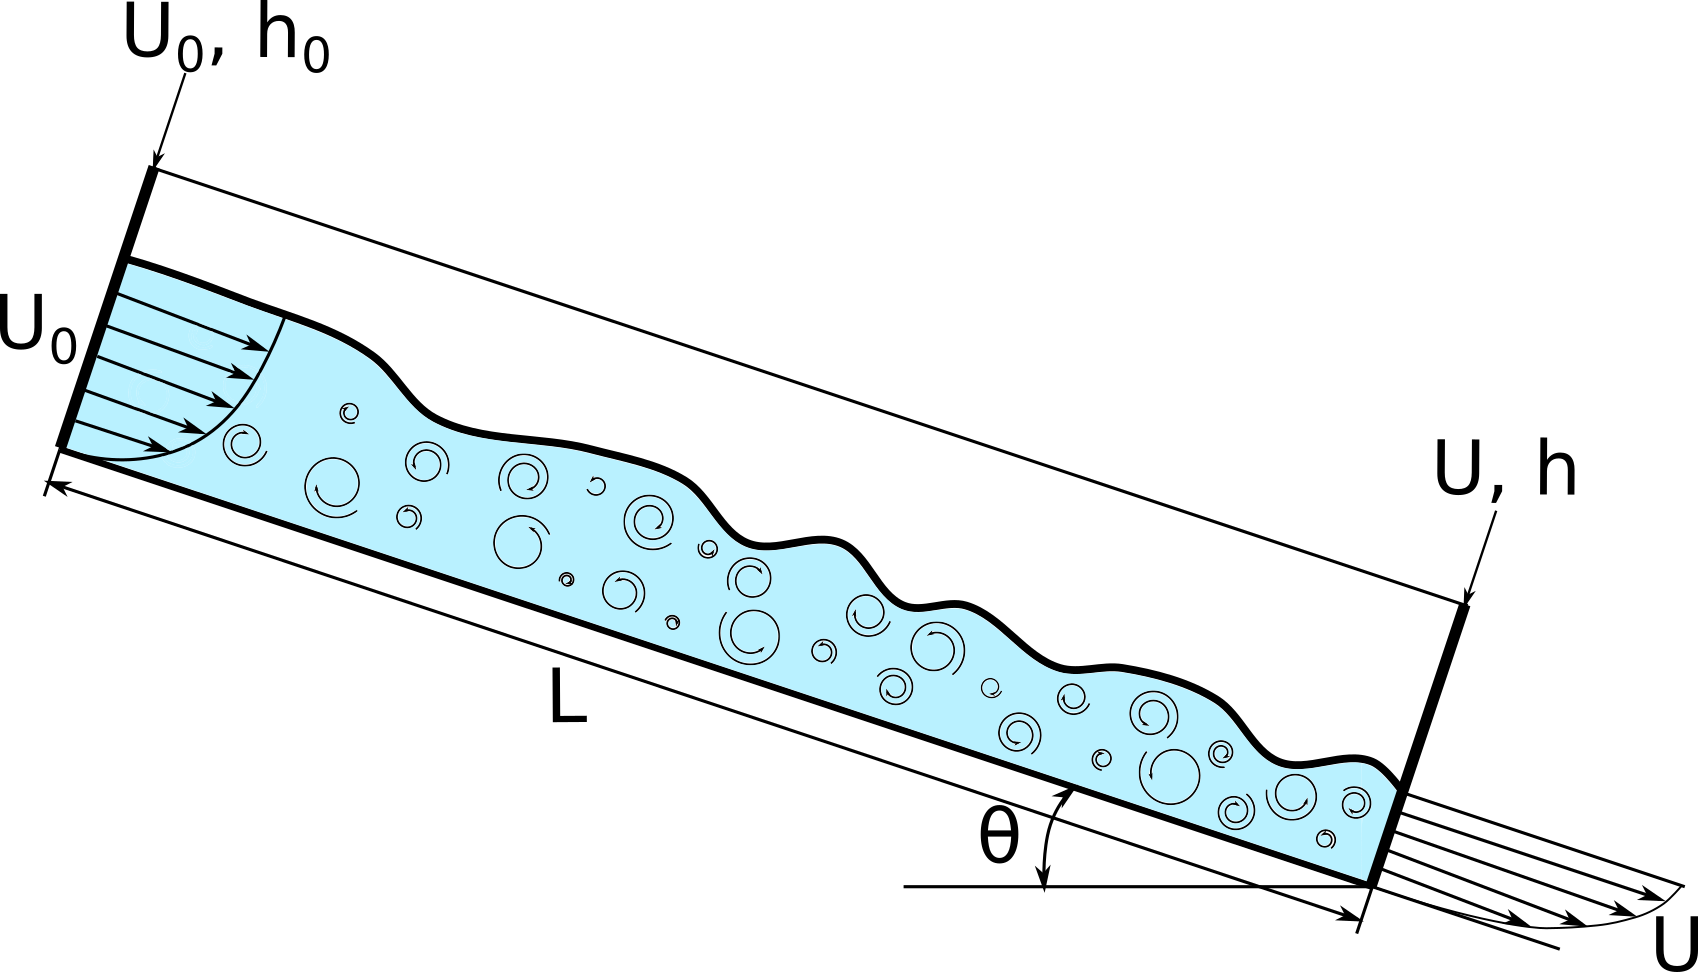
\includegraphics[width=10.5 cm]{NIIMexLinearUProfileInlet.png}
\caption{Schematic diagram of the experimental chute.\label{NIIMexLinearUProfileInlet}}
 
\end{figure}   
 

The experiment was carried out in a stationary mode. Stationarity was provided by a submersible pump ``JEELEX Fekalnik 200'' with a capacity of 200 L per minute. The measurement was carried out using a Pitot tube connected to a ``KORUND-DDN-001M'' pressure sensor with an error of 0.1\%. Measurement points were spaced every 0.5 mm. A 10 s average was used for each measurement. The water temperature in the experiment was 20 degrees Celsius (room temperature). All temperature-related model coefficients were chosen based on this value. 

%Было проведено 3 серии экспериментов, в которых менялся угол наклона склона, начальная глубина потока, начальный профиль потока, как показано в таблице \ref{tabNIIMexLinear}
Three series of experiments were performed; the initial flow profile, the initial flow depth, the slope angle were varied as shown in Table~\ref{tabNIIMexLinear}~\cite{fluids7030111}, where $u_0$ is the depth-averaged velocity, $h_0$ is the flow depth, $\theta$ is the slope inclination angle.

%\begin{table}[H]
%	\caption{Параметры расчётов}
%	\label{tabNIIMexLinear}
%	\begin{center}
%		\begin{tabular}{ | c | c | c | } 
%			\hline
%			$u_0$ среднее по глубине, м/с & $h_0$, мм & $\theta$\\
%			\hline
%			1.63 & 4.20 & 25$^\circ$\\
%			2.00 & 4.95 & 28$^\circ$\\
%			1.78 & 3.45 & 33$^\circ$\\
%			\hline
%		\end{tabular}
%	\end{center}
%\end{table}

\begin{table}[H] 
\caption{{Parameters} of the experiments~\cite{fluids7030111}.\label{tabNIIMexLinear}}
\newcolumntype{C}{>{\centering\arraybackslash}X}
\begin{tabularx}{\textwidth}{CCC}
\toprule
    \textbf{$\boldsymbol{u_0}$, m/s}	&    \textbf{$\boldsymbol{h_0}$, mm}	&     \textbf{$\boldsymbol{\theta}$}\\
\midrule
	1.63 & 4.20 & 25$^\circ$\\
	2.00 & 4.95 & 28$^\circ$\\
	1.78 & 3.45 & 33$^\circ$\\
\bottomrule
\end{tabularx}
\end{table}
\unskip

%%%%%%%%%%%%%%%%%%%%%

%ННГУ

\section{Mathematical Model}\label{math_model}

%Для расчёта эксперимента поставленного в НИИ Механики МГУ используются осреднённые по Рейнольдсу уравнения Навье-Стокса. Для получения значений тензора напряжений Рейнольдса используется замыкание в виде $k-\omega\ SST$ модели турбулентности. Положение свободной поверхности потока определяется с использованием метода объёма жидкости VOF (Volume Of Fluid), предложенного Хиртом и Николсом в 1981 году~\cite{Hirt1981}. В данном методе используется величина объёмной доли фазы воды $\alpha$ в ячейке для определения свободной поверхности таким образом, что при $\alpha>0.6$ считается что ячейка заполнена жидкостью, в противном случае~--- воздухом.
The Reynolds-averaged Navier--Stokes equations~\cite{Wilcox2006, Hirsch2007,FerzigerPeric2002} were used to model the experiment carried out at the Research Institute of Mechanics of Lomonosov Moscow State University. The $k-\omega\ SST$ turbulence model~\cite{Menter1993, Menter1994} was used to obtain the values of the Reynolds stress tensor. The position of the free surface of the flow is determined using the VOF (Volume Of Fluid) method suggested by C.W.~Hirt and B.D.~Nichols in 1981~\cite{Hirt1981}. In this method, the volume fraction of water phase $\alpha$ in the cell is used to determine the free surface so that if $\alpha>0.6$, the cell is considered to be filled with liquid, otherwise---to be filled with air.

%Течение в экспериментальной у становке описывается системой из пяти уравнений. Это уравнения Навье-Стокса, осреднённые по Рейнольдсу (уравнение неразрывности и уравнение сохранения импульса). Так же в систему входит уравнение переноса объёмной доли фазы для отслеживания межфазной границы. Замыкают систему уравнения сохранения для турбулентной кинетической энергии и специальной диссипации турбулентной кинетической энергии, которые используются для вычисления напряжений Рейнольдса, возникающих при осреднении уравнений Навье-Стокса.
The flow in the experimental setup is described by a system of five equations \eqref{vofKWSST}. These are the Reynolds-averaged Navier--Stokes equations (continuity equation and momentum conservation equation). The system also includes a transfer equation for the phase volume fraction to track the interface. The system of equations is closed by two equations of conservation of turbulent kinetic energy and a special dissipation of turbulent kinetic energy, which are used to calculate the Reynolds stresses that arise when averaging the Navier--Stokes equations.
\begin{linenomath} 
%MDPI: Please confirm if bold in equations is necessary. Please check the whole paper
%Authors: Bold is not necessary. Removed
\begin{equation}
	\label{vofKWSST}
	\left\{
		\begin{aligned}
			&{\nabla} \cdot \bar{{u}} = 0,\\
			&\frac{\partial \alpha}{\partial t} + {\nabla} \cdot (\bar{{u}} \alpha) = 0,\\
			&\frac{\partial (\rho \bar{{u}})}{\partial t} + {\nabla} \cdot (\rho \bar{{u}} \bar{{u}}) = -{\nabla} \bar{p} + {\nabla} \cdot \bar{{\tau}} + \rho \bar{{f}},\\
			&\frac{\partial (\rho k)}{\partial t} + {\nabla} \cdot (\rho \bar{{u}} k) = \widetilde{P}_k - \beta^*\rho k \omega + {\nabla} \cdot \left( (\mu + \alpha_k \mu_t) {\nabla} k \right),\\
			&\frac{\partial (\rho \omega)}{\partial t}  + {\nabla} \cdot ( \rho \bar{{u}} \omega) = \gamma \rho \dot{s}^2 - \beta \rho \omega^2 + {\nabla} \cdot \left( (\mu + \alpha_\omega \mu_t) {\nabla} \omega \right) + \\
			&2 (1 - F_1) \rho \alpha_{\omega 2} \frac{1}{\omega} {\nabla} k \cdot {\nabla} \omega.
		\end{aligned}
	\right.
\end{equation}
\end{linenomath}

%Здесь ${u}$~--- скорость смеси; $\alpha$~--- объёмная доля выбранной фазы; $\rho$~--- плотность смеси, рассчитываемая по принципу весового среднего; $\bar{ {\tau}} = 2 \mu_{eff} \bar{ {s}}$~--- тензор напряжений, выраженный через тензор скоростей деформации $\bar{ {s}}$, горизонтальной чертой над буквами обозначается осреднение по Рейнольдсу; $\mu_{eff} = \mu + \mu_t$~--- эффективный коэффициент вязкости, сумма молекулярной вязкости и турбулентной, последняя вычисляется по формуле $\mu_t = \rho a_1 k / \max(a_1 \omega,\ b_1 \dot{s} F_2)$; $\bar{p}$~--- давление; $\bar{ {f}}$~--- плотность массовых сил; $k$---плотность турбулентной кинетической энергии; $\omega$---скорость диссипации плотности турбулентной кинетической энергии; $F_1 = F_1(\beta^*, \alpha_{\omega 1})$~--- функция перемешивания ($F_1$ равняется нулю вдалеке от стены и получается $k-\varepsilon$ модель, и переключается на единицу внутри пограничного слоя, реализуя $k-\omega$ модель); $\dot{s}$~--- скорость сдвига (инвариантная мера $\overline{ {s}}$); $F_2 = F_2(\beta^*)$~--- вторая функция перемешивания, $\widetilde{P}_k$~--- ограничитель на нарастание турбулентности в режимах стагнации.
Here, $\alpha$~is the water volume fraction, $\bar{ {\tau}} = 2 \mu_{eff} \bar{ {s}}$~is the stress tensor, $\bar{ {s}}$~is the strain rate tensor, $\mu_{eff} = \mu + \mu_t$~is the effective viscosity, $\mu$~is a molecular viscosity, $\mu_t = \rho a_1 k / \max(a_1 \omega, \ b_1 \dot{s} F_2)$~is a turbulent viscosity, $\bar{ {f}}$~is the density of the body forces, $\bar{ {u}}$~is the mixture velocity, $\rho$~is the mixture density, $\bar{p}$~is the pressure, $\omega$~is the specific dissipation rate of the turbulent kinetic energy, $k$~is the turbulent kinetic energy, $F_1 = \tanh \left( \left( \min\left( \max \left( \frac{\sqrt{k}}{\beta^* \omega y},\ \frac{500 \nu}{y^2 \omega} \right),\ \frac{4 \rho \alpha_{\omega 2} k}{CD_{k \omega} y^2} \right) \right)^4 \right)$~is the blending function ($F_1$ equals zero away from the wall and the model turns into the $k-\varepsilon$ model, while inside the boundary layer $F_1$ equals one and the $k-\omega$ model is realized),  $\dot{s}$~is the strain rate (invariant of $\overline{ {s}}$), $CD_{k\omega} = \max \left( 2 \rho \alpha_{\omega 2} \frac{1}{\omega}  {\nabla} k \cdot  {\nabla} \omega,\ 10^{-10} \right)$, $F_2 = \tanh \left( \left( \max \left( \frac{2 \sqrt{k}}{\beta^* \omega y},\ \frac{500 \nu}{y^2 \omega} \right) \right)^2 \right)$~is the second blending function, and $\widetilde{P}_k = \min (\mu_t  {\nabla} \bar{ {u}} \cdot \left[  {\nabla} \bar{ {u}} + ( {\nabla} \bar{ {u}})^T\right],\ 10 \cdot \beta^* \rho k \omega)$~is the limiter on the growth of turbulence used in stagnation modes. Details can be found in the OpenFOAM package user guide~\cite{OFUG}.
\nomenclature{$u_0$		}{ depth-averaged velocity on the inlet plane of the experiment chute	}
\nomenclature{$h_0$		}{ flow depth on the inlet plane of the experiment chute	}
\nomenclature{$\theta$	}{ inclination angle of the experiment chute }
\nomenclature{$\alpha$	}{ water volume fraction	}
\nomenclature{$\bar{ {\tau}}$	}{ Reynolds-averaged stress tensor	}
\nomenclature{$\bar{ {s}}$		}{ Reynolds-averaged strain rate tensor	}
\nomenclature{$\mu_{eff}$		}{ effective viscosity	}
\nomenclature{$\mu$		}{ molecular viscosity	}
\nomenclature{$\mu_{t}$		}{ turbulent viscosity	}
\nomenclature{$\bar{ {f}}$		}{ Reynolds-averaged density of body forces	}
\nomenclature{$\bar{ {u}}$		}{ Reynolds-averaged velocity of the mixture	}
\nomenclature{$\rho$		}{ density of the mixture	}
\nomenclature{$\bar{p}$		}{ pressure of the mixture	}
\nomenclature{$\omega$		}{ specific dissipation rate of the turbulent kinetic energy	}
\nomenclature{$k$		}{ 	turbulent kinetic energy }
\nomenclature{$F_1$		}{ first blending function	}
\nomenclature{$\dot{ {s}}$		}{ Reynolds-averaged strain rate	}
\nomenclature{$F_2$		}{ second blending function	}
\nomenclature{$\widetilde{P}_k$ }{ the limiter on the growth of turbulence used in stagnation modes }


%Все константы турбулентной модели рассчитываются по принципу весового среднего между константами $k-\varepsilon$ и $k-\omega$ моделей по принципу $\gamma = \gamma_1 F_1 + \gamma_2 (1 - F_1)$ и т.д. Стандартно константы турбулентной модели задаются следующими значениями~\cite{LaunderSpalding1974, Tahry1983, LaunderMorseRodiSpaldiug1972}:
The turbulence model contains four coefficients: $\alpha_k$, $\alpha_\omega$, $\beta$, $\gamma$. $\alpha_k$, $\alpha_\omega$, $\gamma$ are calculated using the weighted average principle: $\gamma = \gamma_1 F_1 + \gamma_2 (1 - F_1)$. By default, the coefficients of the turbulent model are set by the following values~\cite{LaunderSpalding1974, Tahry1983, LaunderMorseRodiSpaldiug1972}:
\begin{linenomath}
\begin{equation}
	\label{kOmegaSstConstantsInit}
	\begin{aligned}
		\gamma_1 = 5 / 9,\ \ \ \beta_1 = 3 / 40,\ \ \ \alpha_{k1} = 0.85,\ \ \ \alpha_{\omega1} = 0.5,\\
		\gamma_2 = 0.44,\ \ \ \beta_2 = 0.083,\ \ \ \alpha_{k2} = 1,\ \ \ \alpha_{\omega 2} = 0.856,\\
		\beta^* = 0.09,\ \ \ a_1 = 0.31,\ \ \ b_1 = 1.0,\ \ \ c_1 = 10.0.
	\end{aligned}
\end{equation}
\end{linenomath}

\nomenclature{$\alpha_k$ }{ turbulence model closure coefficient }
\nomenclature{$\alpha_{k1}$ }{ turbulence model closure coefficient }
\nomenclature{$\alpha_{k2}$ }{ turbulence model closure coefficient }
\nomenclature{$\alpha_\omega$ }{ turbulence model closure coefficient }
\nomenclature{$\alpha_{\omega1}$ }{ turbulence model closure coefficient }
\nomenclature{$\alpha_{\omega2}$ }{ turbulence model closure coefficient }
\nomenclature{$\beta$ }{ turbulence model closure coefficient }
\nomenclature{$\beta_1$ }{ turbulence model closure coefficient }
\nomenclature{$\beta_2$ }{ turbulence model closure coefficient }
\nomenclature{$\gamma$ }{ turbulence model closure coefficient }
\nomenclature{$\gamma_1$ }{ turbulence model closure coefficient }
\nomenclature{$\gamma_2$ }{ turbulence model closure coefficient }
\nomenclature{$\beta^*$ }{ turbulence model closure coefficient }
\nomenclature{$a_1$ }{ turbulence model closure coefficient }
\nomenclature{$b_1$ }{ turbulence model closure coefficient }
\nomenclature{$c_1$ }{ turbulence model closure coefficient }

The details of the turbulence model description are presented in~\cite{Menter1993, MenterKuntzLangtry2003}.



 
%%%%%%%%%%%%%%%%%%%%%%%%%%%%%%%%%%%%%%%%%%
\section{Methods}\label{sec4}
%ИСП
%\subsection{Используемый численный метод решения ДУЧП}
\subsection{CFD Numerical Method}

%Для реализации трёхмерного многофазного односкоростного подхода использовался решатель interFoam.
To implement the three-dimensional multiphase single-rate approach, the interFoam~\cite{Rusche2003ComputationalFD} solver of OpenFOAM package (v2012, created by Henry Weller in 1989, Bracknell, United Kingdom) was used.

%Используются следующие аппроксимационные схемы:
%\begin{itemize}
%	\item производные по времени $\frac{\partial}{\partial t}$ аппроксимируются с помощью неявного метода Эйлера;
%	\item поток объёмной доли фазы $ {\nabla} \cdot (\bar{ {u}} \alpha)$ аппроксимируется при помощи схемы Ван Лира;
%	\item поток массы смеси $ {\nabla} \cdot (\rho \bar{ {u}} \bar{ {u}})$ аппроксимируется с помощью противопоточной схемы с весами;
%	\item дивергенция тензора вязких напряжений $ {\nabla} \cdot \bar{ {\tau}}$ аппроксимируется с помощью центральной разностной схемы;
%	\item поток турбулентной кинетической энергии $ {\nabla} \cdot (\rho \bar{ {u}} k)$ аппроксимируется противопоточной схемой;
%	\item поток специальной диссипации турбулентной кинетической энергии $ {\nabla} \cdot (\rho \bar{ {u}} \omega)$ используется противопоточная схема;
%	\item оператор градиента $ {\nabla}$ аппроксимируется центрально-разностной схемой;
%	\item оператор Лапласа $ {\nabla}^2$ аппроксимируется центрально-разностной схемой с явной неортогональной коррекцией;
%	\item другие, не перечисленные выше члены описываются с помощью центрально-разностной схемы.
%\end{itemize}

The approximation schemes used in the work are listed below.
\begin{itemize}
	\item The time terms were approximated with first order Euler numerical scheme;
	\item The convection term, the water volume fraction flux term, divergence of the stress tensor term were approximated with second order numerical scheme;
	\item The turbulent kinetic energy flux, the dissipation flux of the specific turbulent kinetic energy term were approximated with first order bounded numerical scheme;
	\item The gradient terms were calculated using Gaussian integration with linear interpolation;
	\item The Laplacian terms were calculated using Gaussian integration with linear interpolation with explicit non-orthogonal correction;
	\item All other terms in the equations were discretized using a central difference numerical scheme.
\end{itemize}

The second order linear upwind scheme used for the convection term is most efficient and accurate for Reynolds Averaged Navier--Stokes (RANS) simulations~\cite{ROBERTSON2015122}.

%Для решения системы уравнений используется алгоритм PIMPLE, являющийся комбинацией алгоритмов PISO (Pressure Implicit with Splitting of Operator) и SIMPLE (Semi-Implicit Method for Pressure-Linked Equations).
The PIMPLE algorithm~\cite{Holzmann2019, Yin2003}, which was developed to run the equations with a large Courant number, was used to solve the system equations. The PIMPLE is a combination of PISO~\cite{Issa1986_2} and SIMPLE~\cite{Issa1986_1} algorithms.

% To solve the system of equations, the PIMPLE~\cite{Holzmann2019, Yin2003} algorithm was used. This algorithm is a combination of the PISO (Pressure Implicit with Splitting of Operator)~\cite{Issa1986_2} and the SIMPLE (Semi-Implicit Method for Pressure-Linked Equations) algorithms~\cite{Issa1986_1}.
%

The conjugate gradient method with preconditioner GAMG is used to solve the system of linear equations for pressure. The GaussSeidel method is used as a smoother. The values for volume fraction of water, velocity, $k$, $\omega$ are defined using smoothSolver and  symGaussSeidel method as a smoother. 

\subsubsection{Definition of the Calculation Domain}

The advantage of mathematical modeling is that the model allows virtual sensors to be placed at any point in the computational domain to measure the values of physical quantities. In the experiment, the physical sensors were placed at the exit from the chute. To compare the results of the experiment and the calculation, the virtual sensors were positioned in the same place.

A section of the experimental chute located between two velocity profile and flow depth measurement points was simulated. 
The simulations were performed for the thick  10~mm part of the chute where the influence of the side walls was small.
The first measured profile was used for the input data for the computational domain. The second one was the object of comparison. 
%
The parallelepiped with a size of 590 mm in length, 10 mm in width, and 10 mm in height was used for the  numerical domain.
%
We tested the effect of grid resolution. Grid convergence was studied for various grid sizes of $290 \times 10 \times 30$, $590 \times 10 \times 60$, $1080 \times 10 \times 120$, and $2160 \times 10 \times 240$. For each run, the output velocity profile was compared with the experimental one using the loss function \eqref{LossFunction}. The values of the loss functions for the last three mesh sizes varied within 0.1\%. Therefore, the number of cells was chosen to be $590 \times 10 \times 60$ for reasons of reducing computer time while maintaining accuracy.

\subsubsection{Initial and Boundary Conditions}

%Были выделены следующие границы расчётной области: дно лотка, боковые стенки лотка, верхняя граница лотка, плоскость на входе в лоток, плоскость на выходе из лотка.
The special boundaries for numerical domain were defined: the chute bottom, the chute sides, the upper border for numerical domain, and the inlet and outlet planes.

%Были заданы следующие граничные условия:
%\begin{itemize}
%	\item дно лотка: является твёрдой стенкой с условием прилипания потока; 
%	\item боковые стенки лотка: задано условие нулевого градиента для реализации отсутствия влияния стенок на поток;
%	\item верхняя граница лотка: смешанное условие с заданием атмосферного давления, и условия отсутствия притока среды через данную границу, отток происходит по принципу нулевого градиента;
%	\item входная плоскость: заданы фиксированные значения объёмной доли воды и профиля скорости потока;
%	\item выходная плоскость: для всех величин установлено условие нулевого градиента.
%\end{itemize}
The following boundary conditions were set:

\begin{itemize}
    \item The solid wall with the no-slip condition was used for the chute bottom;
    \item The zero gradient condition was used for the chute side;
    \item The mixed condition with atmospheric pressure was used for the upper border of numerical domain, no inflow through the border and outflow according to zero gradient condition and fixed value condition for $k$ and $\omega$;
    \item The fixed values were used for inlet plane for water volume fraction, velocity profile, $k$ and $\omega$ values;
    \item The zero gradient condition was used for outlet plane.
\end{itemize}

The mathematical formulation of the listed initial and boundary conditions is presented in the OpenFOAM user manual~\cite{OFUG}.

%High Reynolds wall functions used in $k-\omega\ SST$ turbulence model.
The average value of $Y+$ was 17 which satisfied the model of wall functions. The nutkWallFunction was used for boundary condition for the wall, which provides a wall constraint on the turbulent viscosity, based on the turbulent kinetic energy for both low- and high-Reynolds number turbulence models.

%Начальные условия в задаче таковы, что объём полностью заполнен неподвижным воздухом и подаётся жидкость через входную плоскость, спустя время поток устанавливается и снимаются замеры на выходной плоскости для сравнения с экспериментальными данными. Поток считается установившимся спустя 5 секунды.

The initial conditions in the problem are set so that the volume is completely filled with stationary air and the liquid flows in through the inlet plane. After a while, the flow is established and measurements are taken on the outlet plane for comparison with the experimental data. The time step $dt$ is equal to 0.001 s. The flow is considered steady after 5 s.


%%%%%%%%%%%%%%%%%%%%Перенести в раздел с оптимизацией


%При оптимизации коэффициентов турбулентной модели минимизируется корень из среднеквадратического отклонения вычисленного профиля скорости потока на выходной плоскости от экспериментального профиля:



%%%%%%%%%%%%%%%%%%%%%%%%%%%%%%%%%%%%%%%%%%


%Для расчёта эксперимента НИИ Механики МГУ была рассчитана часть экспериментального лотка, находящаяся между двумя точками замера профиля скорости и глубины потока. Расчёт проводился для срединной полоски лотка толщиной 10~мм, где влияние боковых стенок незначительно. Первый измеренный профиль подавался на вход расчётной области, второй являлся объектом сравнения. Геометрия расчётной области представляет собой параллелепипед длинной 590~мм, шириной 40~мм, и глубиной 10~мм. Количество ячеек составило 590х10х60.



%Более детальное описание математической модели можно найти в книге Ферцигера и Перича~\cite{FerzigerPeric2002}.



%ННГУ
\subsection{Global Optimization Problem Statement}
The Globalizer software (Lobachevsky University) was used to solve the optimization problem.

Let us assume that the choice of some set of values of the model parameters is determined by the values of vector $y=(y_1,y_2,...,y_N)$ and the quality of the model corresponding to a given value of the vector of parameters is described by the function $\varphi(y)$. Let us call this function the optimization criterion: a decrease in the criterion value corresponds to a better mathematical model. Additionally, assume that some requirements must be satisfied to guarantee the applicability of the model. Meeting these requirements is usually formulated as the condition for the vector $y$ to belong to the hyperinterval $D$,
%MDPI: Is italic necessary?
%Authors: Italic is not necessary. Removed
\begin{linenomath}
\begin{equation}
D=\{a_i \leq y_i \leq b_i, \; 1 \leq i \leq N\}.
\end{equation}
\end{linenomath}

\nomenclature{$y = (y_1, ..., y_N)$ }{ vector of parameter}
\nomenclature{$\varphi(y)$		}{ objective function	}
\nomenclature{$D$	}{ hyperinterval	}


So far, the process of choosing the optimal set of the model parameters corresponds to a global optimization problem of the kind:
\begin{linenomath}
\begin{equation}\label{main_problem}
\begin{aligned}
    & \varphi(y^\ast)=\min{\left\{\varphi(y):y\in D\right\}},\\
    & D=\left\{y\in \text{R}^N: a_i\leq y_i \leq b_i, 1\leq i \leq N\right\}.
\end{aligned}
\end{equation}
\end{linenomath}

When optimizing the coefficients of the turbulent model, the Root-Mean-Square Error (RMSE) of differentiation of the calculated flow velocity profile and the experimental one on the outlet plane is taken into account. 
%MDPI: Please confirm if bold in equations is necessary. Please check the whole paper
%Authors: Bold is not necessary. Removed
\begin{linenomath}
\begin{equation}
	\label{LossFunction}
	 {L_{RMSE}} = \sqrt{\frac{\sum\limits_{i=1}^{N} \left( u_{EXP}^i - u_{k-\omega\ SST}^i \right)^2}{N}}
\end{equation}
\end{linenomath}
is minimized. 
%где $h$~--- глубина потока на выходной плоскости.
Here, $u_{EXP}^i$ is the horizontal component of velocity at the control point obtained by experiment, and $u_{k-\omega\ SST}^i$  is the horizontal component of velocity at the control point calculated by computational fluid dynamic (CFD), $N$ is the number of comparison points for the horizontal component of velocity over the flow depth at the outlet plane (right cross-section displayed in Figure \ref{NIIMexLinearUProfileInlet}). Approximately 10 comparison points are used. Their number is determined by the number of measurements performed in the experiment and varies depending on the change in the flow depth at different chute inclination angles. The points are evenly distributed in depth for the operation of measurement tools used in the experiment.
\nomenclature{$N$		}{ number of measuring points of velocity over the flow depth at the outlet plane	}
\nomenclature{$u^i_{EXP}$		}{ horizontal component of velocity at the control point obtained by experiment	}
\nomenclature{$u^i_{k-\omega}\ SST$		}{ horizontal component of velocity at the control point calculated by CFD	}
\nomenclature{$ {L_{RMSE}}$		}{ loss function	}


We will consider the loss function (\ref{LossFunction}) as the objective function $\varphi(y)$ in the global optimization problem (\ref{main_problem}). 
The problems considered are characterized by the fact that the objective function $\varphi(y)$ is not defined analytically; there is only an algorithm for computing its values at the points of the domain $D$. In this case, one search trial corresponds to one computation according to the model and is a time- consuming operation~\cite{Kalyulin2017,Paulavicius2020}.

Multi-extremal optimization problems have much higher computation costs for solving them as compared to other types of optimization problems since the global optimum is an integral characteristic of the problem being solved and requires investigating the whole search domain. As a result, the search for the global optimum is reduced to constructing some coverage (grid) in some range of parameters and choosing the optimal function value on this grid. The amount of computations may be reduced by constructing a non-uniform coverage of the search domain: the grid should be dense enough in the vicinity of the global optimum and less dense far away from the sought solution

The assumption that the objective function $\varphi(y)$ satisfies the Lipschitz condition
\begin{linenomath}
\begin{equation}
\left|\varphi(y_1)-\varphi(y_2)\right|\leq L\left\|y_1-y_2\right\|,\; y_1,y_2 \in D, \; 0<L<\infty,
\end{equation}
\end{linenomath}
is a typical and is used in many global optimization methods~\cite{Sergeyev2013,Evtushenko2013,Jones2009,Zilinskas2010}.
The assumption of this kind is natural enough for many applied problems since the relative variations of the function characterizing the process being simulated cannot usually exceed some threshold imposed by the limited energy of variation. The question of estimating the Lipschitz constant values unknown {\textit a priori} arising here can be resolved by introducing some additive schemes~\cite{Strongin2020,Strongin2020_1}.
\nomenclature{$L$		}{ Lipschitz constant	}

There are several ways to adapt efficient one-dimensional algorithms for solving multidimensional problems (see, e.g.,~\cite{Sergeyev2017,Zilinskas2014}). In this study we apply the dimensionality reduction using Peano curve $y(x)$ continuously mapping the unit interval [0,1] onto the $n$-dimensional cube
\begin{linenomath}
\begin{equation}
\left\{y\in R^N: -2^{-1}\leq y_i \leq 2^{-1}, 1 \leq i \leq N\right\}=\left\{y(x):0\leq x \leq 1 \right\}.
\end{equation}
\end{linenomath}

Algorithms for constructing Peano-type space filling curves and the corresponding theory are considered in detail in~\cite{Strongin2000,Sergeyev2013}.

By using this kind of mapping, the multivariate problem~(\ref{main_problem}) could be reduced to a univariate problem
\begin{linenomath}
\begin{equation}
\varphi(y^\ast)=\varphi(y(x^\ast))=\min{\left\{\varphi(y(x)): x\in[0,1]\right\}}.
\end{equation}
\end{linenomath}

An important property of such mapping is that if the function $\varphi(y)$ in the domain $D$ satisfies the Lipschitz condition, then the function $\varphi(y(x))$ on the interval $[0,1]$ will satisfy a uniform H{\"o}lder condition
\begin{linenomath}
\begin{equation}
\left|\varphi(y(x_1))-\varphi(y(x_2))\right|\leq H\left|x_1-x_2\right|^{1/N},
\end{equation}
\end{linenomath}
where the H{\"o}lder constant $H$ is linked to the Lipschitz constant $L$ by the relation $H=2L\sqrt{N+3}$~\cite{Strongin2000}.
\nomenclature{$H$		}{ H{\"o}lder constant	}


Therefore, we can consider minimization of univariate function
\begin{linenomath}
\begin{equation}
f(x)=\varphi(y(x)), \;\; x\in[0,1],
\end{equation}
\end{linenomath}
satisfying the H{\"o}lder condition.
\nomenclature{$y(x)$		}{ Peano curve	}
\nomenclature{$f(x) = \varphi(y(x))$		}{ univariate function	}


\newpage


\subsection{The Global Search Algorithm}\label{GSA}

The algorithm for solving the problem (\ref{main_problem}) involves constructing a sequence of points $x^k$, where the values of the objective function $z^k = f(x^k)=\varphi(y(x^k))$ are calculated. Let us call the process of calculating the function value (including the construction of an image $y^k=y(x^k)$) the ``trial'', and the pair $(y^k, z^k)$, the ``trial result''. The set of pairs $\left\{(y^k, z^k), 0\leq k\leq n\right\}$ makes up the search data collected using the method after carrying out $n$ steps. The rules that determine the work of the \textit{global search algorithm} are as follows.

The first two trials are performed at the boundary points of the segment $[0,1]$, i.e., $x^0 = 0$ and $x^1 = 1$. The values $z^0 = f(x^0)$ and $z^1 = f(x^1)$ of the objective function are calculated, and the counter $k = 1$ is set. A next trial point $x^{k+1}, k \geq 1,$ is chosen using the following rules.

Step 1. Renumber points of the set $X_k=\{x^0,\dots,x^k\} $ with subscripts in increasing order of coordinate values, i.e.,
\begin{linenomath}
\begin{equation}
0=x_0<x_1<\dots <x_{k-1}<x_{k}=1.
\end{equation}
\end{linenomath}

\nomenclature{$X_k=\{x^0,\dots,x^k\} $ }{ set of the trial points }

Note that hereinafter superscripts are used to denote the iteration number, and subscripts are used to number the points in order.

Step 2. Supposing that  $z_i=f(x_i), \; 1\leq i \leq k$, calculate values 
\begin{linenomath}
\begin{equation}\label{mu}
\mu = \max_{1\leq i \leq k}\frac{\left|z_i-z_{i-1}\right|}{\Delta_i},
\end{equation}
\end{linenomath}
\begin{linenomath}
\begin{equation}
M = \left\{
   \begin{array}{lr}
     r\mu, & \mu > 0,\\
     1, & \mu = 0,
   \end{array}
\right.
\end{equation}
\end{linenomath}
where the real number $r>1$ is the method input parameter, and $\Delta_i=\left(x_i-x_{i-1}\right)^{1/N}$.

\nomenclature{$z^k = f(x^k)$ }{ value of the objective function }
\nomenclature{$M$		}{ adaptive estimation of the Lipschitz constant }
\nomenclature{$r>0$		}{ method parameter	}

Step 3. For each interval $(x_{i-1}, x_i), \; 1\leq i \leq k,$ calculate a characteristic according to the following formula
\begin{equation}\label{R}
R(i)=\Delta_i+\frac{(z_i-z_{i-1})^2}{M^2\Delta_i}-2\frac{z_i+z_{i-1}}{M},1 \leq i \leq k.
\end{equation}

\nomenclature{$R(i)$		}{ characteristic of the $i$-th search interval}

Step 4. Select the interval $(x_{t-1},x_t)$ corresponding to the maximum characteristic
\begin{equation}\label{MaxR}
R(t)=\max{\left\{R(i): 1 \leq i \leq k \right\}}.
\end{equation}

Step 5. Execute the new trial at the point $x^{k+1}\in(x_{t-1},x_t)$, calculated using the following formula
\begin{equation}\label{NewX}
x^{k+1} = \frac{x_t+x_{t-1}}{2} - \mathrm{sign}(z_t-z_{t-1})\frac{1}{2r}\left[\frac{\left|z_t-z_{t-1}\right|}{\mu}\right]^N.
\end{equation}

The algorithm stops when $\Delta_t<\epsilon$, where $\epsilon>0$ is the preset accuracy. For estimation of the global optimum, values
\begin{linenomath}
\begin{equation}
f_k^\ast=\min_{0\leq i \leq k}f(x^i), \ x_k^\ast=\arg \min_{0\leq i \leq k}f(x^i),
\end{equation}
\end{linenomath}
are chosen.

A rigorous proof of this algorithm's convergence is provided in~\cite{Strongin2000}. 
%The modifications taking into account existence of inequality constraints in the problem and the information about the objective function derivative are given in~\cite{RefBarkalov,RefGergel1996,RefGergel1997}

\newpage

\subsection{Construction of the Objective Function Approximation}

\subsubsection{The Use of Neural Networks}

There are no universal rules for the choice of the neural network topology to solve a particular problem. However, in~\cite{Cybenko1989} the Kolmogorov theorem has been generalized and it was proved that any continuous function of $N$ variables can be approximated by a three-layered artificial feedforward neural network with one hidden layer and an error backpropagation algorithm as a learning one with any degree of precision. This theorem is called the Universal Approximation Theorem or the Cybenko theorem~\cite{Hassoun1995}.

Neural networks as approximators were implemented in many machine learning libraries.
In the present study, MLPRegressor class from scikit-learn machine learning library was used  to construct the objective function approximation. It implements a multi-layer perceptron (MLP), which is learned using error backpropagation without activation function in the output layer~\cite{Nielsen1989}. MLPs have demonstrated an ability to find approximate solutions for very complex problems.

A MLP with one hidden layer with a scalar output is shown in Figure \ref{fig1}.

\begin{figure}[H]
 
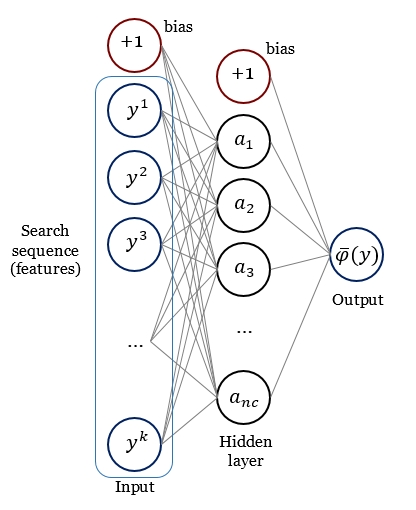
\includegraphics[width=5 cm]{perceptron.jpg}
\caption{Three-layer perceptron with scalar output.\label{fig1}}
 
\end{figure}
 

The left layer called the input layer consists of a set of neurons $y_i, \; i=\overline{1,k}$ representing the input signals (the values of variables). Each neuron in the hidden layer transforms the values from the previous layer with weighted linear summing 
\begin{linenomath}
\begin{equation}
w_1 y_1 + w_2 y_2+...+w_k y_k+bias,
\end{equation}
\end{linenomath}
where $w_i$ are the weights of the neurons and $bias$ is a special weight, which does not include a factor in the form of an input value. Next, the value obtained is transformed into an output (predicted) value of the layer with a transmission function (the \textit{activation function}). The output layer receives the values from the last hidden layer and transforms them into the output values. The network was trained by the error backpropagation method.

We used a three-layered neural network for solving the approximation problem due to the following reasons. From the theoretical point of view, such a network will be sufficient to approximate the function with a high accuracy. From the practical point of view, the use of deep neural networks here will be redundant, because the set of trial results used to build the approximation is small and will not be sufficient to train a deep network.

\subsubsection{Selection of the Model Parameters}

The choice of the solver, the activation function, the value of the regularization parameter, the number of neurons in the hidden layer, etc., are the variable adjustment parameters of the neural network.
For example, for small sets of the multidimensional data, the ``lbfgs'' solver was demonstrated to be better and faster. This solver is a modification of the Broyden--Fletcher--Goldfarb--Shanno algorithm~\cite{Nocedal2006} and belongs to the quasi-Newton methods. All numerical experiments were carried out using this algorithm.
The sigmoidal functions (logistic or hyperbolic tangent) were used as the neuron activation functions.
The number of neurons in each layer and the regularization parameter (alpha) were adjusted in the experiments and depended on a particular problem.

In the experiments conducted, we chose the following network architecture:

 

\begin{verbatim}
    model = MLPRegressor(activation='logistic',
	solver='lbfgs',
	alpha=0.001,
	hidden_layer_sizes=(20,),
	max_iter=5000,
	tol=10e-6,
	random_state=10)
\end{verbatim}


\subsection{The Use of Approximations in Solving the Optimization Problem}\label{GSA_Appr}

In the present study, we applied the following method of using the objective function approximation in the optimization problems: to construct the objective function approximation using the accumulated search information, to find the minimum of the approximation, and to repeat this process, either until the computation resources are exhausted or until the convergence is achieved.

The method proposed will make sense either in the case when the amount of the search information accumulated is large enough (that allows constructing a relatively precise approximation of a multi-extremal function) or in the case when the problem is similar to a local extremum search problem.
The first case corresponds to the final stage of search and can be interpreted as a method of refining the current solution. However, if the objective function is time-consuming, it is impossible to conduct a large enough number of trials. This is where we will encounter an exhaustion of computing resources.

The second case implies constructing a good approximation based on a relatively small number of trials and, in fact, includes an assumption on a weak multi-extremality of the objective function that matches well with the problem considered within the framework of the present study.
 
The global search algorithm using the objective function approximation can be formulated as follows.
Let us assume that the available resources allow for $K_{max} = K_1 + K_2$ trials to be performed.

At the first stage, $k = K_1$ trials are performed using the core global search algorithm from Section \ref{GSA}.
In the course of performing the first stage, a set of the trial results $\Omega = \left\{(y^k, \varphi(y^k)), 0\leq k\leq K_1\right\}$ necessary to construct the objective function approximation is accumulated.

At the second stage, the algorithm works using the approximation. To compute the point $y^{k+1}$ of the next $(k+1)^{\rm th}$ trial, the following operations are performed.

%Описание работы алгоритма
Step 1. Using the set of the trial results $\Omega$ formed in the course of the algorithm execution, to construct an approximation of the objective function $\overline{\varphi}(y)$;

Step 2. Using the core global search algorithm from Section \ref{GSA} to find the global minimum of the function $\overline{\varphi}(y)$ and to use this value as the next trial point, i.e., $y^{k+1} = \arg \min_{y \in D} \overline{\varphi}(y)$;

Step 3. If either the condition $k>K_{max}$ or the condition $\left\|y^k - y^{k+1}\right\| \leq \epsilon$ is satisfied, to stop the algorithm.
Else, to perform the trial at the point $y^{k+1}$, to store its result in the set $\Omega$, to increment the trial counter $k = k+1$, and to proceed to Step 1.

\nomenclature{$\epsilon > 0$		}{ search accuracy	}
\nomenclature{$\Omega $ }{ set of the trial results }
\nomenclature{$\overline{\varphi}(y)$ }{ approximation of the objective function }

The algorithm proposed here ensures the convergence to the global solution in the case if $K_1$ trials executed at the first stage are sufficient to construct an approximation of the objective function reflecting the main features of its behavior adequately.

%пример работы алгоирмта на тестовой задаче?

%%%%%%%%%%%%%%%%%%%%%%%%%%%%%%%%%%%%%%%%%%

%\subsection{Loss function definition}

%%%%%%%%%%%%%%%%%%%%%%%%%%%%%%%%%%%%%%%%%%
\section{Results}\label{sec5}

%Описание оборудования и программного обеспечения, которое было задействовано при проведении экспериментов.

%Результаты расчетов

%Иллюстрации

%Сравнение нескольких разных решений (это можно перенести и в следующую секцию)

The simulations were conducted using the supercomputer of Lobachevsky University of Nizhni Novgorod (operated under the Linux CentOS 7.2 operation system). Each supercomputer node included two Intel Sandy Bridge E5-2660 2.2 GHz processors, 64 Gb RAM. The central processor unit had 8 cores. 
The global optimization methods considered in the present work were implemented in C++ using GCC 5.5.0 compiler and Open MPI v4.1.1. To construct the objective function approximations using a neural network, scikit-learn machine learning library from Python 3.9 was applied. 
To numerically solve the problem described in Section \ref{math_model}, the open source CFD software OpenFOAM v2012~\cite{OpenFOAM} was~used.

%В процессе оптимизации исследовались такие константы, как $\beta^*$, $a_1$, $\alpha_{k 1,2}$, $\alpha_{\omega 1,2}$, которые регулируют скорость диссипации турбулентной кинетической энергии, напряжения Рейнольдса, поток диффузии турбулентной кинетической энергии, поток диффузии диссипации турбулентной кинетической энергии, соответственно.
Before starting the calibration, a small study of the significance of each of the 12~coefficients of the turbulent model was carried out. As a result, it was revealed that the coefficients $\beta^*$, $a_1$, $\alpha_{k 1,2}$, and $\alpha_{\omega 1,2}$ make the most significant contribution to the calculation results. It was decided to calibrate these coefficients. These coefficients determine the dissipation rate of turbulent kinetic energy, the Reynolds stress, the diffusion fluxes of turbulent kinetic energy, and the specific dissipation rate. The coefficient $\beta^*$ is used in the mixing functions that describe the mechanism for switching between the $k-\varepsilon$ and $k-\omega$ models. The coefficient $a_1$ determines the turbulent viscosity. $\alpha_{k 1,2}$ characterize the diffusion flux of the kinetic energy of turbulence. $\alpha_{\omega 1,2}$ characterize the diffusion flow by the specific rate of dissipation of the kinetic energy of turbulence.

%Начальные значения коэффициентов были заданы следующими:
The initial values of the coefficients are 
\begin{linenomath}
\begin{equation}
	\begin{aligned}
		\beta^* = 0.09;\ \ \ a_1 = 0.31;\ \ \ \alpha_{k 1} = 0.85;\ \ \ \alpha_{\omega 1} = 0.5; \ \ \ \alpha_{k 2} = 1.0;\ \ \ \alpha_{\omega 2} = 0.856.
	\end{aligned}
\end{equation}
\end{linenomath}

One calculation of the objective function for given values of parameters took 15 min in average with the use of 8 MPI-processes per node. 

The optimal values of parameters were adjusted for pairs, the values of the remaining parameters were fixed. 
First, a pair of the most important parameters $\beta^*$ and $a_1$ was selected. 
To investigate the optimization problem posed, both possible approaches to solving it were applied: without the use of the objective function approximation  and with the use of the approximation.

In the first experiment, the global search algorithm described in Section \ref{GSA} was applied without the use of approximation. 
The parameters of the method were set as follows: $r = 3$ and $\epsilon = 10^{-3}$. 
In 24 h, 100 iterations of the algorithm were performed; the required accuracy was not achieved. 

In the second experiment, the approach described in Section \ref{GSA_Appr} was applied to solve the same problem.
First, $K_1 = 30$ iterations of global search algorithm were performed. 
Afterwards, the algorithm employing the approximation with the neural network was started. 
A total of $K_1 + K_2 = 65$ iterations of the algorithm were performed, after that the algorithm stopped on accuracy. 
As a result, the best value  of the objective function 0.375 was found. 
The total search time was reduced to 16 h, which ensured a more accurate solution for the problem in a reasonable amount of time.

The trial points and the approximating function plotted according to these points using the neural network are presented in Figure~\ref{NN_100_point} (the parameters $\beta^*$ and $a_1$ were varied). Several local minima are clearly visible.
Our analysis showed good agreement between the regression model and experimental data.
The $R^2$ score and the RMSE between the model predictions and the simulated results are equal to 0.976 and 0.098, respectively.


\begin{figure}[H]
 
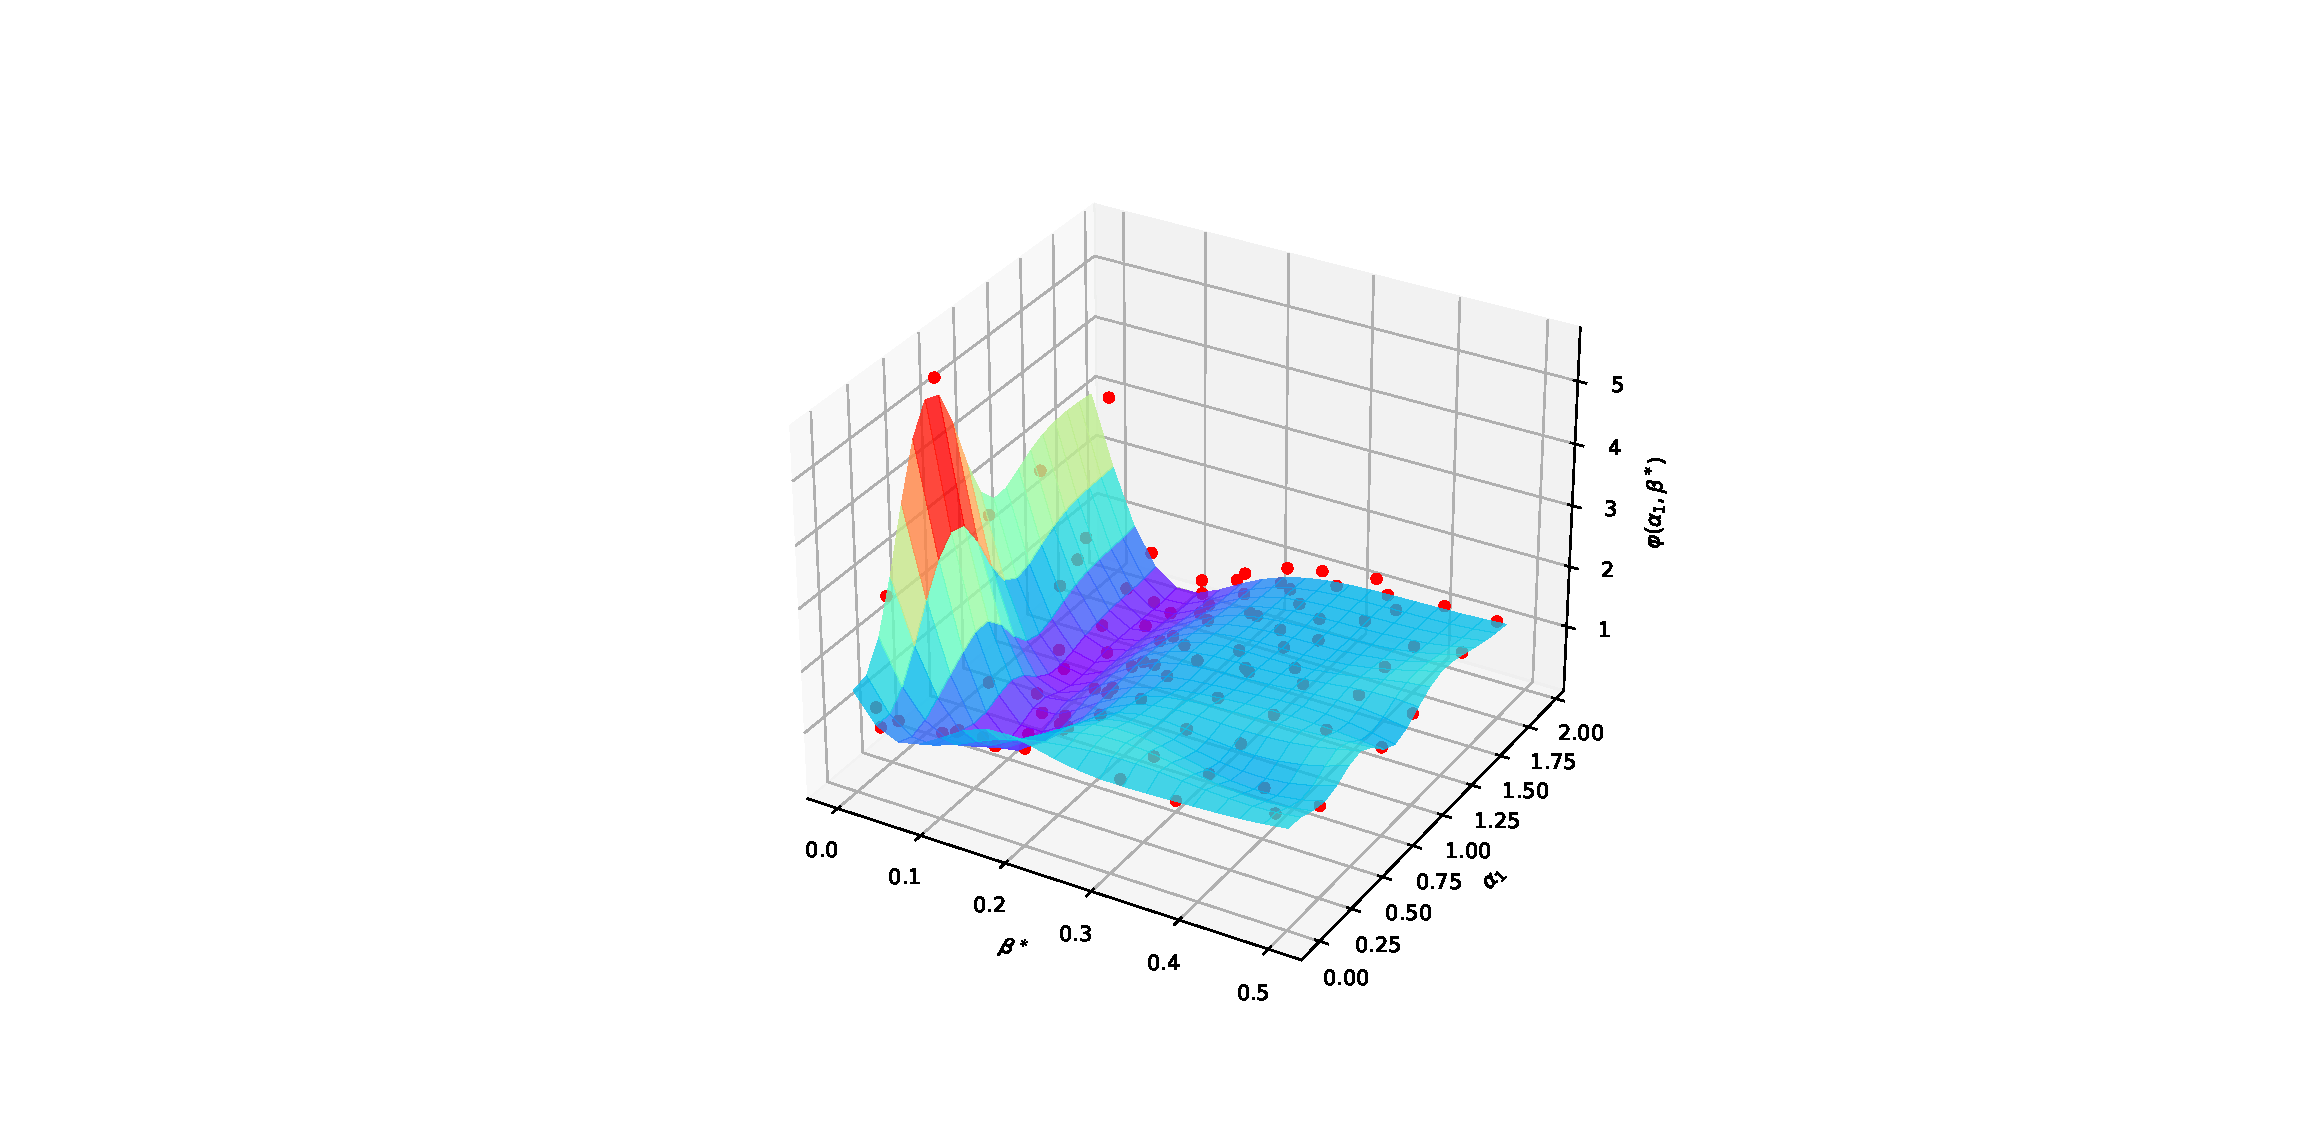
\includegraphics[width=0.6\linewidth]{NN_100_point_.pdf}
\caption{Objective 
%MDPI: please check if different colors need explanation, if yes, please add.
%Authors: Different colors does not need explanation
function values (red points) and the approximation plot constructed using the neural network (parameters $\beta^*$ and $a_1$ were varied).\label{NN_100_point}}
 
\end{figure}   
 

The best values of parameters $\beta^*$ and $a_1$ found were fixed, and then optimization in parameters $\alpha_{k1}, \alpha_{\omega1}$, and $\alpha_{k2}, \alpha_{\omega2}$ was performed. 
However, no significant improvement of the objective function by optimizing on these parameters was achieved: the value of 0.365 was obtained.


%На рисунках ~\ref{NN_100_point1} и ~\ref{NN_100_point2} приведены изображение функций, полученные с помощью аппроксимации задачи нейросетью, обученной на 100 точках испытания, варьировались соответсвенно пары параметров $\alpha_{k1} $,  $\alpha_{\omega1} $ и $\alpha_{k2} $, $\alpha_{\omega2} $.
%
%\begin{figure}[H]
%\begin{center}
%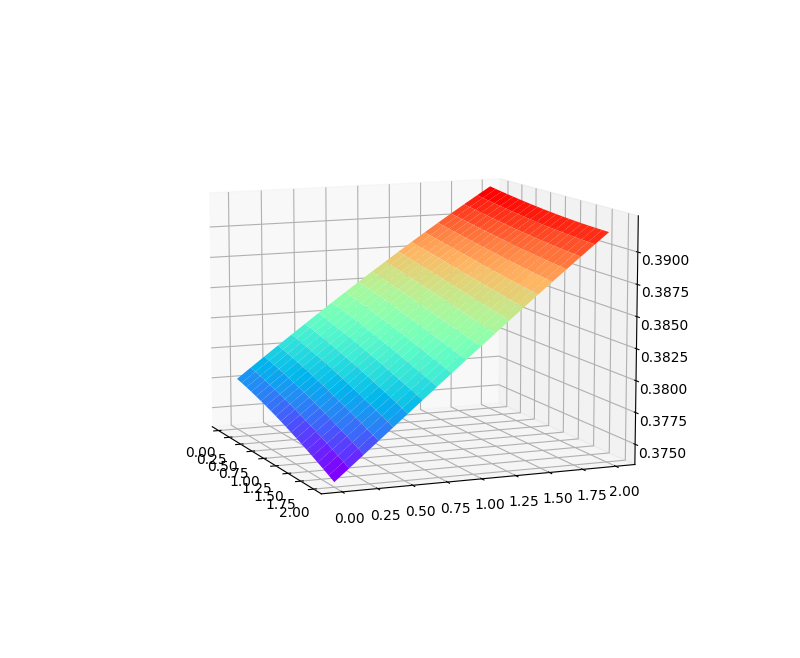
\includegraphics[width=1.0\linewidth]{ NN_100_point_1.png}
%\caption{Изображение функции, полученной с помощью аппроксимации задачи нейросетью, обученной на 100 точках испытания, варьировались параметры $\alpha_{k1} $ и $\alpha_{\omega1} $}
%\label{NN_100_point1}
%\end{center}
%\end{figure}
%
%\begin{figure}[H]
%\begin{center}
%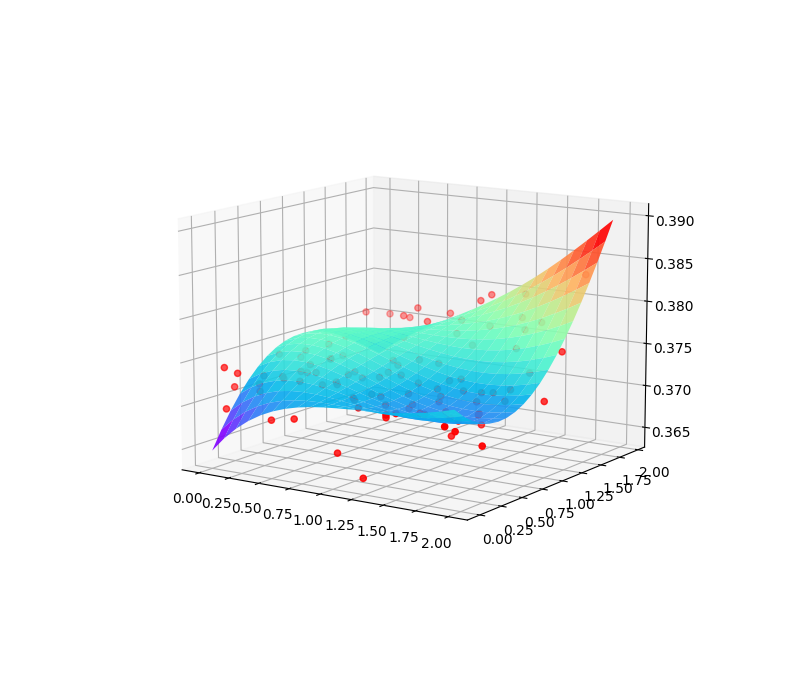
\includegraphics[width=1.0\linewidth]{ NN_100_point_tanh_alpha2_0.0001_.png}
%\caption{Изображение функции, полученной с помощью аппроксимации задачи нейросетью, обученной на 100 точках испытания, варьировались параметры $\alpha_{k2} $ и $\alpha_{\omega2} $}
%\label{NN_100_point2}
%\end{center}
%\end{figure}

%После калибровки значения коэффициентов стали следующими:
%The optimized values of the coefficients:
As a final result, the following values of the coefficients of the model were obtained:

\begin{linenomath}
\begin{equation}
	\begin{aligned}
		\beta^* = 0.117;\ \ \ a_1 = 1.84;\ \ \ \alpha_{k 1} = 1.999;\\
		\alpha_{\omega 1} = 0.062; \ \ \ \alpha_{k 2} = 1.241;\ \ \ \alpha_{\omega 2} = 0.003.
	\end{aligned}
\end{equation}
\end{linenomath}

%Были получены следующие профили скорости на выходной плоскости для различных углов наклона лотка, как показано на рис.~\ref{NIIMexUProfilesKWSSTGlob}
Figure~\ref{NIIMexUProfilesKWSSTGlob} shows the resulting velocity profiles $\bar{ {u_x}}$ as a function of flow depth $h$ on the exit plane for various slope angles.

\begin{figure}[H]
\begin{adjustwidth}{-\extralength}{0cm}
\centering
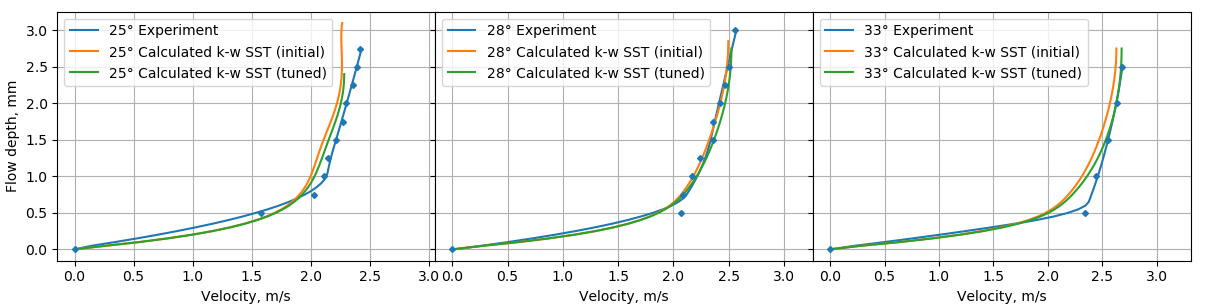
\includegraphics[width=18 cm]{UProfilesKWSSTGlob1.png}
\end{adjustwidth}
\caption{The 
%MDPI: please check if the blue diamond need explanation, if yes, please add.
%Authors: Blue diamond does not need explanation.
comparison graphs of the experimental velocity profile and the calculated velocity profile using the standard values of the $k-\omega\ SST$ turbulence model coefficients and the calculated velocity profile with calibrated values of the coefficients for different slope inclination angles.\label{NIIMexUProfilesKWSSTGlob}}
\end{figure}  

%Калибровка привела к следующей минимизации функции потерь~\eqref{LossFunction}, показанной в таб.~\ref{tabLossFunctionMinimize}
During the process of calibration, the minimization of the loss function~\eqref{LossFunction} was achieved, as shown in Table~\ref{tabLossFunctionMinimize}.

%\begin{table}[H]
%	\caption{Минимизация функции потерь}
%	\label{tabLossFunctionMinimize}
%	\begin{center}
%		\begin{tabular}{ | c | m{0.3\textwidth} | m{0.3\textwidth} | } 
%			\hline
%			Угол наклона лотка& Начальное значение функции потерь & Минимизированное значение функции потерь\\
%			\hline
%			25$^\circ$ & 0.165 & 0.155\\
%			\hline
%			28$^\circ$ & 0.085 & 0.128\\
%			\hline
%			33$^\circ$ & 0.150 & 0.089\\
%			\hline
%		\end{tabular}
%	\end{center}
%\end{table}
\begin{table}[H] 
\caption{Loss function values obtained during the minimization process.\label{tabLossFunctionMinimize}}
\newcolumntype{C}{>{\centering\arraybackslash}X}
\begin{tabularx}{\textwidth}{CCC}
\toprule
    \textbf{Slope Inclination Angle} & \textbf{Initial Loss Function Value} & \textbf{Minimized Loss Function Value}\\
\midrule
    25$^\circ$ & 0.165 & 0.155\\
    28$^\circ$ & 0.085 & 0.128\\
    33$^\circ$ & 0.150 & 0.089\\
\bottomrule
\end{tabularx}
\end{table}
 

%На рисунке \ref{NIIMexUProfilesKWSSTGlob} и в таблице \ref{tabLossFunctionMinimizeKE} можем видеть, что для двух углов наклона из трёх мы видим уменьшение расхождения расчётного профиля скорости с экспериментальным. Оптимизация по трём экспериментам одновременно (их функции потерь суммировались) использовалась с целью избежать переобучения модели, так как при использовании одного эксперимента, может быть достигнуто почти идеальное совпадение расчётного профиля скорости с экспериментальным, которое не воспроизводится на других экспериментах. Так же стоит отметить, что расхождение профиля скорости в области вблизи дна обусловлено погрешностью измерений в эксперименте, так как замер скорости с помощью трубки Пито, используемой в данном эксперименте, в непосредственной близости ото дна затруднён.
Figure~\ref{NIIMexUProfilesKWSSTGlob} and Table~\ref{tabLossFunctionMinimize} show a decrease in the discrepancy between the calculated velocity profile and the experimental one for two out of three experiments. Optimization for the three experiments combined (their loss functions were summarized) was used in order to avoid the model overfitting. In one experiment, an almost perfect coincidence of the calculated velocity profile with the experimental one was achieved, which was not reproduced in other experiments. It should also be noted that the divergence of the velocity profile in the region near the chute bottom is due to the measurement error in the experiment, since it is difficult to measure the velocity with the Pitot tube used in this experiment in the immediate vicinity of the bottom.

The minimum value for the objective function was obtained in the case of the slope angle of 33 degrees. One calculation of the objective function for the given parameters took 15 min in average using 8 MPI processes on a node of the Lobachevsky University supercomputer. Total computation time was 24 h.

%%%%%%%%%%%%%%%%%%%%%%%%%%%%%%%%%%%%%%%%%%
\section{Discussion}\label{sec6}

%В процессе работы над оптимизацией коэффициентов турбулентной модели мы столкнулись с рядом задач: создание интерфейса взаимодействия программного обеспечения Глобалайзер и пакета OpenFOAM; в процессе оптимизации мы столкнулись с проблемой переобучением модели; было проведено исследование наилучшей функции потерь и др.
When working on the optimization of the turbulent model coefficients, we faced a number of tasks: creating an interface for automatic interaction between the Globalizer software and the OpenFOAM package; in the process of optimization, we encountered the overfitting problem; and the study of the best loss function was carried out, etc.

%Создание интерфейса взаимодействия между Globalizer и OpenFOAM потребовало использования библиотеки pyFoam для подготовки прогонов расчетов. С помощью скрипта этой библиотеки pyFoamPrepareCase.py в расчетные варианты были записаны новые значения констант модели турбулентности, предложенной программой Globalizer. Далее проводился расчет в параллельном режиме и оценка полученного результата. Результат оценивался с помощью python-скрипта, который сравнивал полученный профиль скорости с экспериментальным.
Creating an interaction interface between Globalizer and OpenFOAM required the use of the pyFoam library to prepare calculation runs. Using the script of this library pyFoamPrepareCase.py, new values of the turbulent model coefficients proposed by the Globalizer software were written into the calculation cases. Next, the calculation was carried out in parallel mode and the result was evaluated using a python script that compared the obtained velocity profile with the experimental one.

A study of various loss functions has been carried out. The loss functions that estimate the absolute error of the velocity profile and the relative error were compared. The relative loss function actually penalizes the area near the bottom more, however, optimization using this loss function did not show significant improvements in the result. This behavior of the calculation is not due to the shortcomings of the numerical model, but rather due to the impossibility of taking velocity values correctly in the region very close to the bottom of the chute. It should be noted that measurements at the point closest to the bottom can have a significant error, due to the measurement method used (the Pitot tube). However, most of the profile was measured quite accurately, since for each measurement point in this stationary experiment, time averaging of 10 s was used. As a result of this study, it was decided to use the absolute loss function, since it showed the best optimization result.

We performed three experiments to avoid overfitting. It was noticed that when optimizing for one velocity profile, the algorithm perfectly calibrated the model, but for other experiments, the result was much worse. When optimizing for three experiments at once, this effect was avoided. The use of the obtained values of the coefficients for fluid flows that are close in dimensionless characteristics will allow a more accurate calculation to be made. However, when generalized to such canonical flows as air flow around different profiles, the use of the obtained values of the turbulent model coefficients is unlikely to show the best result.

\newpage

This study is part of a larger research effort related to the modeling of currents on the slopes of mountains. These flows are very difficult to study, since they are turbulent multi-phase flows of a non-Newtonian fluid on slopes of complex geometry. For such flows, the use of turbulent models using standard values of coefficients does not predict the flow in the best way. It is necessary to calibrate the turbulence model coefficients or create new turbulence models. We are considering both options. Moreover, a new turbulent model is being developed based on the neural network. However, the use of neural networks requires hybrid computing clusters, which is not always possible. As a result, it is important to be able to obtain a solution of sufficient accuracy using the classical turbulent model. This problem requires the calibration of the coefficients, which was done in this work for the Newtonian medium. Optimization algorithms were developed and tested, which can later be used to calibrate the coefficients of any turbulent models. The next stage of the study is to set up an experiment with a non-Newtonian fluid and calibrate the coefficients of the turbulent model according to the developed algorithm.

%Отметим также, что при поиске оптимальных параметров модели проводилась оптимизация сначала по параметрам $\beta^*$ and $a_1$, затем – по параметрам $\alpha_{k1}, \alpha_{\omega1}$, and $\alpha_{k2}, \alpha_{\omega2}$. Данный способ позволил найти хорошее решение за приемлемое время. Поиск глобального минимума сразу по всем варьируемым параметрам потребовал бы на порядки большего числа испытаний и, соответственно, времени. Указанный эффект ключевым образом отличает задачи глобальной оптимизации от задач на локальный экстремум, в которых затраты растут не столь быстро.
We also note that when searching for the optimal model parameters, optimization was carried out first with respect to the parameters $\beta^*$ and $a_1$, then optimization in $\alpha_{k1}, \alpha_{\omega1}$, and $\alpha_{k2}, \alpha_{\omega2}$ was performed. This approach makes it possible to find a good solution in a reasonable amount of time.
The search for a global optimum for all parameters at once would require orders of magnitude more trials and time.
This effect is a key difference between global optimization and local optimization problems, in which the costs do not grow as fast.

%С точки зрения решения вычислительно трудоемкой задачи оптимизации с целевой функцией вида черный ящик представляет интерес сравнение использованного метода решения задачи, в котором целевая функция аппроксимировалась нейросетью, с распространенными методами, использующими аппроксимации на основе кригинга. Методы данного класса хорошо работают в задачах с небольшим числом локальных экстремумов, однако в существенно многоэкстремальных задачах вычислительные затраты значительно возрастают.
In terms of solving a time-consuming optimization problem with a black-box objective function, it is interesting to compare the method used for solving the problem, which uses objective function approximation by a neural network, with the methods that use kriging-based approximations.
Methods of this class work well in problems with a small number of local extrema.
However, in essentially multi-extremal problems the computational costs (number of objective function evaluations required for solving the problem) increase significantly.


%%%%%%%%%%%%%%%%%%%%%%%%%%%%%%%%%%%%%%%%%%
\section{Conclusions}\label{sec7}

In this work, a two-phase flow in a chute was simulated using the interFoam solver, the URANS mathematical model, and the $k-\omega\ SST$ turbulence model. In the optimization process, six coefficients were investigated in pairs, which make the greatest contribution to the value of turbulent viscosity.

The results of calculating the velocity profiles were compared with experimental data obtained at the Research Institute of Mechanics, Moscow State University, at different sections depending on the angle of inclination of the chute. The search for the optimal coefficients of the turbulence model was performed by minimizing the objective function of the divergence of the velocity profile in the chute. % - RMSE.

The search for the global minimum of the objective function was performed using the global search algorithm implemented in the Globalizer software~\cite{globalizerSystem}. In addition, a fully connected neural network with one hidden layer was used to approximate the values of the objective function by the values of the coefficients in the turbulence model. The MLPRegressor class from the scikit-learn library was used to build the objective function approximation.

Based on the results of the study, the following conclusions were drawn.

It is good practice to calibrate the turbulence model coefficients if necessary to improve the accuracy of the calculations. As shown in the present study, it is possible to improve the accuracy by up to 10\%.

To perform optimization, at least two, or preferably three datasets should be used. Otherwise, an overfitted model may result.
Using a neural network to predict the CFD calculation significantly reduced the optimization time while maintaining the quality of the resulting solution.

 

The developed calibration algorithm is reliable and can be applied to other models. The algorithm has such advantages as a parallel mode, it can be used to search not only for local, but also for global minima, and can optimize several parameters at once. According to the results of the study, the Globalizer software has performed quite well and will be used in further work.

The OpenFOAM software also shows good results due to code modularity and good documentation. These advantages have made it easier to write a software module for the interaction between the optimizer and OpenFOAM. OpenFOAM also has a high degree of parallelization and can be used to solve a fairly wide range of tasks.

In the present work, an interdisciplinary approach was utilized, which helped us to find the optimal values of six turbulence model parameters using the OpenFOAM open platform and the Globalizer.  
In the future, it is planned to continue improving the turbulent models, including the development of a turbulent model based on a neural network. The Globalizer software will be used to optimize the model parameters.

\nomenclature{NNR		}{ Neural Network Regression	}
\nomenclature{RMSE		}{ Root-Mean-Square Error	}
\nomenclature{CFD }{ Computational Fluid Dynamic }
\nomenclature{RANS }{ Reynolds-Averaged Navier-Stokes equations }
\nomenclature{PISO }{ Pressure Implicit with Splitting of Operator }
\nomenclature{SIMPLE }{ Semi-Implicit Method for Pressure-Linked Equations }
\nomenclature{PIMPLE }{ combination of PISO and SIMPLE }  

%%%%%%%%%%%%%%%%%%%%%%%%%%%%%%%%%%%%%%%%%%
\vspace{6pt} 

%%%%%%%%%%%%%%%%%%%%%%%%%%%%%%%%%%%%%%%%%%
%% optional
%\supplementary{The following supporting information can be downloaded at:  \linksupplementary{s1}, Figure S1: title; Table S1: title; Video S1: title.}

% Only for the journal Methods and Protocols:
% If you wish to submit a video article, please do so with any other supplementary material.
% \supplementary{The following supporting information can be downloaded at: \linksupplementary{s1}, Figure S1: title; Table S1: title; Video S1: title. A supporting video article is available at doi: link.}

%%%%%%%%%%%%%%%%%%%%%%%%%%%%%%%%%%%%%%%%%%
\authorcontributions{Conceptualization, K.B. and D.R. (Daniil Ryazanov); methodology, D.R. (Daria Romanova) and K.B.; software, I.L., D.R. (Daniil Ryazanov), M.U., and  D.R. (Daria Romanova); validation,  D.R. (Daria Romanova) and I.L.; formal analysis, S.S., M.U.; investigation, S.S.; resources, I.L.; data curation, D.R. (Daria Romanova) and M.U.; writing---original draft preparation, K.B., S.S. and D.R. (Daria Romanova); writing---review and editing, D.R. (Daniil Ryazanov); visualization, I.L.; supervision, S.S.; project administration, K.B.; funding acquisition, S.S. All authors have read and agreed to the published version of the manuscript.}

\funding{This research was supported by the Ministry of Science and Higher Education of the Russian Federation, agreement No 075-15-2020-808.}

\institutionalreview{Not applicable.}

\informedconsent{Not applicable.}

\dataavailability{Not applicable.} 

\acknowledgments{The authors consider it their duty to acknowledge the contribution of  Victor Gergel (14.01.1955--29.06.2021), who initiated this interdisciplinary study.}

\conflictsofinterest{The authors declare no conflicts of interest.} 

%%%%%%%%%%%%%%%%%%%%%%%%%%%%%%%%%%%%%%%%%%
%% Optional
%\sampleavailability{Samples of the compounds ... are available from the authors.}

%% Only for journal Encyclopedia
%\entrylink{The Link to this entry published on the encyclopedia platform.}

%\abbreviations{Abbreviations}{
%The following abbreviations are used in this manuscript:\\

%\noindent 
%\begin{tabular}{@{}ll}
%MDPI & Multidisciplinary Digital Publishing Institute\\
%DOAJ & Directory of open access journals\\
%TLA & Three letter acronym\\
%LD & Linear dichroism
%\end{tabular}
%}

%%%%%%%%%%%%%%%%%%%%%%%%%%%%%%%%%%%%%%%%%%
%% Optional
\appendixtitles{no} % Leave argument "no" if all appendix headings stay EMPTY (then no dot is printed after "Appendix A"). If the appendix sections contain a heading then change the argument to "yes".

%%\appendixstart
%%\appendix
%%\section[\appendixname~\thesection]{}\label{app}%Nomenclature%List of symbols and abbreviations


%\subsection[\appendixname~\thesubsection]{}
%The appendix is an optional section that can contain details and data supplemental to the main text---for example, explanations of experimental details that would disrupt the flow of the main text but nonetheless remain crucial to understanding and reproducing the research shown; figures of replicates for experiments of which representative data are shown in the main text can be added here if brief, or as Supplementary Data. Mathematical proofs of results not central to the paper can be added as an appendix.

%$\alpha_{k1,2}$, $\alpha_{\omega1,2}$, $\beta_{1,2}$, $\gamma_{1,2}$, $\beta^*$, $a_1$, $b_1$, $c_1$ & turbulence model constant \\

%%\vspace{-6pt}

%%\begin{table}[H] 
%%\caption{\hl{Nomenclature}.\label{A:tab1}} 
%MDPI: Please consider using  Nomenclature format instead, Not Appendix A, Table A1
%Authors: The nomenclature has been revised. But we think it looks better in tables. Therefore, we have left the tables here as a comment with double commenting symbol (&&).
%%\newcolumntype{C}{>{\centering\arraybackslash}X}
%%\begin{tabularx}{\textwidth}{ll}
%%\toprule
%%$u_0$		& depth-averaged velocity on the inlet plane of the experiment chute	\\
%%$h_0$		& flow depth on the inlet plane of the experiment chute	\\
%%$\theta$	& inclination angle of the experiment chute \\
%%$\alpha$	& water volume fraction	\\
%%$\bar{ {\tau}}$	& Reynolds-averaged stress tensor	\\
%%$\bar{ {s}}$		& Reynolds-averaged strain rate tensor	\\
%%$\mu_{eff}$		& effective viscosity	\\
%%$\mu$		& molecular viscosity	\\
%%$\mu_{t}$		& turbulent viscosity	\\
%%$\bar{ {f}}$		& Reynolds-averaged density of body forces	\\
%%$\bar{ {u}}$		& Reynolds-averaged velocity of the mixture	\\
%%$\rho$		& density of the mixture	\\
%%$\bar{p}$		& pressure of the mixture	\\
%%$\omega$		& specific dissipation rate of the turbulent kinetic energy	\\
%%$k$		& 	turbulent kinetic energy \\
%%$F_1$		& first blending function	\\
%%$\dot{ {s}}$		& Reynolds-averaged strain rate	\\
%%$F_2$		& second blending function	\\
%%$\widetilde{P}_k$ & the limiter on the growth of turbulence used in stagnation modes \\
%%$\alpha_k$ & turbulence model closure coefficient \\
%%$\alpha_{k1}$ & turbulence model closure coefficient \\
%%$\alpha_{k2}$ & turbulence model closure coefficient \\
%%$\alpha_\omega$ & turbulence model closure coefficient \\
%%$\alpha_{\omega1}$ & turbulence model closure coefficient \\
%%$\alpha_{\omega2}$ & turbulence model closure coefficient \\
%%$\beta$ & turbulence model closure coefficient \\
%%$\beta_1$ & turbulence model closure coefficient \\
%%$\beta_2$ & turbulence model closure coefficient \\
%%$\gamma$ & turbulence model closure coefficient \\
%%$\gamma_1$ & turbulence model closure coefficient \\
%%$\gamma_2$ & turbulence model closure coefficient \\
%%$\beta^*$ & turbulence model closure coefficient \\
%%$a_1$ & turbulence model closure coefficient \\
%%$b_1$ & turbulence model closure coefficient \\
%%$c_1$ & turbulence model closure coefficient \\
%%$y = (y_1, ..., y_N)$ & vector of parameter\\
%%$\varphi(y)$		& objective function	\\
%%$D$	& hyperinterval	\\
%%$N$		& number of measuring points of velocity over the flow depth at the outlet plane	\\
%%$u^i_{EXP}$		& horizontal component of velocity at the control point obtained by experiment	\\
%%$u^i_{k-\omega}\ SST$		& horizontal component of velocity at the control point calculated by CFD	\\
%%$ {L_{RMSE}}$		& loss function	\\
%%$L$		& Lipschitz constant	\\
%%$H$		& H{\"o}lder constant	\\
%%$y(x)$		& Peano curve	\\
%%$f(x) = \varphi(y(x))$		& univariate function	\\
%%$X_k=\{x^0,\dots,x^k\} $ & set of the trial points \\
%%$z^k = f(x^k)$ & value of the objective function \\
%%$M$		& adaptive estimation of the Lipschitz constant \\
%%$R(i)$		& characteristic of the $i$-th search interval\\
%%$r>0$		& method parameter	\\
%%$\epsilon > 0$		& search accuracy	\\
%%$\Omega $ & set of the trial results \\
%%$\overline{\varphi}(y)$ & approximation of the objective function \\
%%\bottomrule
%%\end{tabularx}
%%\end{table}

%%\begin{table}[H] 
%%\caption{\hl{List of abbreviations.}\label{A:tab2}} %MDPI: Please consider using  Abbreviations format instead, Not Appendix A, Table A2. 
%%\newcolumntype{C}{>{\centering\arraybackslash}X}
%%\begin{tabularx}{\textwidth}{ll}
%%\toprule
%%NNR		& Neural Network Regression	\\
%%RMSE		& Root-Mean-Square Error	\\
%%CFD & Computational Fluid Dynamic \\
%%RANS & Reynolds-Averaged Navier-Stokes equations \\
%%PISO & Pressure Implicit with Splitting of Operator \\
%%SIMPLE & Semi-Implicit Method for Pressure-Linked Equations \\
%%PIMPLE & combination of PISO and SIMPLE \\  
%%\bottomrule
%%\end{tabularx}
%%\end{table}

%\section[\appendixname~\thesection]{}
%All appendix sections must be cited in the main text. In the appendices, Figures, Tables, etc. should be labeled, starting with ``A''---e.g., Figure A1, Figure A2, etc.

\printnomenclature

%%%%%%%%%%%%%%%%%%%%%%%%%%%%%%%%%%%%%%%%%%
\begin{adjustwidth}{-\extralength}{0cm}
%\printendnotes[custom] % Un-comment to print a list of endnotes

\reftitle{References}

% Please provide either the correct journal abbreviation (e.g., according to the “List of Title Word Abbreviations” http://www.issn.org/services/online-services/access-to-the-ltwa/) or the full name of the journal.
% Citations and References in Supplementary files are permitted provided that they also appear in the reference list here. 

%=====================================
% References, variant A: external bibliography
%=====================================
%\bibliography{your_external_BibTeX_file}
\begin{thebibliography}{999}

\bibitem[Pendin and Fomenko(2015)]{Pendin2015}
Pendin, V.; Fomenko, I.
\newblock {\em Landslide Hazard Assessment and Prediction Methodology};  2015; 
  p. 320. 
  %MDPI: Please add the name of the publisher and the location (city, country) of it. Or please add website and accessed date(before receive date 6 July 2022)
  %Authors: Information is not available

\bibitem[Froude and Petley(2018)]{Froude2018}
Froude, M.J.; Petley, D.N.
\newblock Global fatal landslide occurrence from 2004 to 2016.
\newblock {\em Nat. Hazards Earth Syst. Sci.} {\bf 2018}, {\em
  18},~2161--2181.
\newblock {{https://doi.org/10.5194/nhess-18-2161-2018}}.

\bibitem[Hungr(2005)]{hungr2005landslide}
Hungr, O.
\newblock {\em Landslide Risk Management: Proceedings of the International
  Conference on Landslide Risk Management, Vancouver, BC,  Canada, 31 May--3 June
  2005}; Balkema: Leiden, NY, USA,  2005.

\bibitem[Kharchenko and Shvarev(2020)]{Harch2020}
Kharchenko, S.; Shvarev, S.
\newblock Forecasting of Landslide Hazards in the Vicinity of Krasnaya Polyana
  Basing on Liniar Discriminatory Analysis.
\newblock {\em Vestnik Moskow State Univ. Ser. 5 Geography.} {\bf 2020},  22--33.
\newblock
  Available online:  \url{https://vestnik5.geogr.msu.ru/jour/article/view/668?locale=en_US}  accessed on 1 may 2022).
  %MDPI: Please add volume and doi link.  Or please add website and accessed date(before receive date 6 July 2022)
  %Authors: Fixed

\bibitem[Bernander \em{et~al.}(2016)Bernander, Kullingsj\"{o}, Gylland,
  Bengtsson, Knutsson, Pusch, Olofsson, and Elfgren]{Bernander2016}
Bernander, S.; Kullingsj\"{o}, A.; Gylland, A.S.; Bengtsson, P.E.; Knutsson,
  S.; Pusch, R.; Olofsson, J.; Elfgren, L.
\newblock Downhill progressive landslides in long natural slopes: Triggering
  agents and landslide phases modeled with a finite difference method.
\newblock {\em Can. Geotech. J.} {\bf 2016}, {\em 53},~1565--1582.
\newblock {{https://doi.org/10.1139/cgj-2015-0651}}.

\bibitem[Gao \em{et~al.}(2007)Gao, Jian-li, and Chang-yu]{liu2007application}
Gao, L.; Jian-li, D.; Chang-yu, L.
\newblock The application of finite volume method to modeling landslide motion.
\newblock {\em Adv. Earth Sci.} {\bf 2007}, {\em 22},~1129--1133.

\bibitem[Liu \em{et~al.}(2020)Liu, Su, Zhang, Iqbal, Hu, and Dong]{Liu2020}
Liu, Z.; Su, L.; Zhang, C.; Iqbal, J.; Hu, B.; Dong, Z.
\newblock Investigation of the dynamic process of the Xinmo landslide using the
  discrete element method.
\newblock {\em Comput. Geotech.} {\bf 2020}, {\em 123},~103561.
\newblock {{https://doi.org/10.1016/j.compgeo.2020.103561}}.

\bibitem[Piegari \em{et~al.}(2006)Piegari, Cataudella, Di~Maio, Milano, and
  Nicodemi]{piegari2006cellular}
Piegari, E.; Cataudella, V.; Di~Maio, R.; Milano, L.; Nicodemi, M.
\newblock A cellular automaton for the factor of safety field in landslides
  modeling.
\newblock {\em Geophys. Res. Lett.} {\bf 2006}, {\em 33}, L01403.

\bibitem[Hirt and Nichols(1981)]{Hirt1981}
Hirt, C.; Nichols, B.
\newblock Volume of fluid ({VOF}) method for the dynamics of free boundaries.
\newblock {\em J. Comput. Phys.} {\bf 1981}, {\em
  39},~201--225. 
  %MDPI: Ref. 9 and 68 are same.  please, either replace the duplicate with a new reference, or we will help remove the duplicate and rearrange the reference order.
  %Authors: Fixed
\newblock {{https://doi.org/10.1016/0021-9991(81)90145-5}}.

\bibitem[Naaim \em{et~al.}(2002)Naaim, Furdada, and Mart{\'{\i}}nez]{Naaim2002}
Naaim, M.; Furdada, G.; Mart{\'{\i}}nez, H.
\newblock Calibration and application of the {MN}2D dynamics model to the
  avalanches of Las Le{\~{n}}as (Argentina).
\newblock {\em Nat. Hazards Earth Syst. Sci.} {\bf 2002}, {\em
  2},~221--226.
\newblock {{https://doi.org/10.5194/nhess-2-221-2002}}.

\bibitem[Pitman \em{et~al.}(2003)Pitman, Nichita, Patra, Bauer, Sheridan, and
  Bursik]{Pitman2003}
Pitman, E.B.; Nichita, C.C.; Patra, A.; Bauer, A.; Sheridan, M.; Bursik, M.
\newblock Computing granular avalanches and landslides.
\newblock {\em Phys. Fluids} {\bf 2003}, {\em 15},~3638--3646.
\newblock {{https://doi.org/10.1063/1.1614253}}.

\bibitem[Oda \em{et~al.}(2011)Oda, Moriguchi, Kamiishi, Yashima, Sawada, and
  Sato]{Oda2011}
Oda, K.; Moriguchi, S.; Kamiishi, I.; Yashima, A.; Sawada, K.; Sato, A.
\newblock Simulation of a snow avalanche model test using computational fluid
  dynamics.
\newblock {\em Ann. Glaciol.} {\bf 2011}, {\em 52},~57--64.
\newblock {{https://doi.org/10.3189/172756411797252284}}.

\bibitem[Yamaguchi \em{et~al.}(2017)Yamaguchi, Takase, Moriguchi, Terada, Oda,
  and Kamiishi]{Yamaguchi2017}
Yamaguchi, Y.; Takase, S.; Moriguchi, S.; Terada, K.; Oda, K.; Kamiishi, I.
\newblock Three-dimensional nonstructural finite element analysis of snow
  avalanche using non-Newtonian fluid model.
\newblock {\em Trans. Jpn. Soc. Comput. Eng. Sci.} {\bf 2017}, {\em 2017}, 20170011.
\newblock {{https://doi.org/10.11421/jsces.2017.20170011}}.

\bibitem[Agustsdottir(2019)]{IceThesKatr}
Agustsdottir, K.H.
\newblock The Design of Slushflow Barriers: Laboratory Experiments. Doctoral Dissertation, University of Iceland,  Reykjavik, Iceland, 
\newblock  2019.

\bibitem[Jones(2019)]{IceThesJon}
Jones, R.
\newblock The Design of Slushflow Barriers: CFD Simulations. Doctoral Dissertation,
\newblock  2019.
%MDPI: Please add Degree-Granting University and Location of University(city and countrty).  Or please add website and accessed date(before receive date 6 July 2022)
%Authors: Fixed
\newblock
  Available online:  \url{http://hdl.handle.net/1946/34502}  accessed on 1 may 2022).

\bibitem[Jaedicke \em{et~al.}(2006)Jaedicke, Kern, Gauer, Baillifard, and
  Platzer]{Jaedicke2006}
Jaedicke, C.; Kern, M.; Gauer, P.; Baillifard, M.A.; Platzer, K.
\newblock Chute Experiments on Slushflow Dynamics. In  Proceedings of the   2006 International Snow Science Workshop,  Telluride, CO, USA, 1--6 October 2006.
\newblock  

\bibitem[Cheung \em{et~al.}(2011)Cheung, Oliver, Prudencio, Prudhomme, and
  Moser]{Cheung2011}
Cheung, S.H.; Oliver, T.A.; Prudencio, E.E.; Prudhomme, S.; Moser, R.D.
\newblock Bayesian uncertainty analysis with applications to turbulence
  modeling.
\newblock {\em Reliab. Eng.  Syst. Saf.} {\bf 2011}, {\em
  96},~1137--1149.
\newblock {{https://doi.org/10.1016/j.ress.2010.09.013}}.

\bibitem[Guillas \em{et~al.}(2014)Guillas, Glover, and
  Malki-Epshtein]{Guillas2014}
Guillas, S.; Glover, N.; Malki-Epshtein, L.
\newblock Bayesian calibration of the constants of the turbulence model for a
  {CFD} model of street canyon flow.
\newblock {\em Comput. Methods Appl. Mech. Eng.} {\bf
  2014}, {\em 279},~536--553.
\newblock {{https://doi.org/10.1016/j.cma.2014.06.008}}.

\bibitem[Edeling \em{et~al.}(2014{\natexlab{a}})Edeling, Cinnella, and
  Dwight]{Edeling2014a}
Edeling, W.; Cinnella, P.; Dwight, R.
\newblock Predictive {RANS} simulations via Bayesian Model-Scenario Averaging.
\newblock {\em J. Comput. Phys.} {\bf 2014}, {\em 275},~65--91.
\newblock {{https://doi.org/10.1016/j.jcp.2014.06.052}}.

\bibitem[Edeling \em{et~al.}(2014{\natexlab{b}})Edeling, Cinnella, Dwight, and
  Bijl]{Edeling2014b}
Edeling, W.; Cinnella, P.; Dwight, R.; Bijl, H.
\newblock Bayesian estimates of parameter variability in the
  k{\textendash}$\upepsilon$ turbulence model.
\newblock {\em J. Comput. Phys.} {\bf 2014}, {\em 258},~73--94.
\newblock {{https://doi.org/10.1016/j.jcp.2013.10.027}}.

\bibitem[de~Zordo-Banliat \em{et~al.}(2020)de~Zordo-Banliat, Merle, Dergham,
  and Cinnella]{deZordoBanliat2020}
de~Zordo-Banliat, M.; Merle, X.; Dergham, G.; Cinnella, P.
\newblock Bayesian model-scenario averaged predictions of compressor cascade
  flows under uncertain turbulence models.
\newblock {\em Comput.  Fluids} {\bf 2020}, {\em 201},~104473.
\newblock {{https://doi.org/10.1016/j.compfluid.2020.104473}}.

\bibitem[Matsui \em{et~al.}(2021)Matsui, Perez, Kelly, Tani, and
  Jemcov]{Matsui2021}
Matsui, K.; Perez, E.; Kelly, R.; Tani, N.; Jemcov, A.
\newblock Calibration of Spalart-Allmaras model for simulation of corner flow
  separation in linear compressor cascade.
\newblock {\em J. Glob. Power Propuls. Soc.} {\bf 2021},
  pp. 1--16.
\newblock {{https://doi.org/10.33737/jgpps/135174}}.

\bibitem[Xiao and Cinnella(2019)]{Xiao2019}
Xiao, H.; Cinnella, P.
\newblock Quantification of model uncertainty in {RANS} simulations: A review.
\newblock {\em Prog. Aerosp. Sci.} {\bf 2019}, {\em 108},~1--31.
\newblock {{https://doi.org/10.1016/j.paerosci.2018.10.001}}.

\newpage

\bibitem[Karpatne \em{et~al.}(2017)Karpatne, Ebert{-}Uphoff, Ravela, Babaie,
  and Kumar]{GeoML}
Karpatne, A.; Ebert{-}Uphoff, I.; Ravela, S.; Babaie, H.A.; Kumar, V.
\newblock Machine Learning for the Geosciences: Challenges and Opportunities. \emph{IEEE Trans. Knowl. Data Eng.}  \textbf{2018}, \emph{31}, 1544--1554. %MDPI: We revised journal information, please confirm
%\newblock {\em CoRR} {\bf 2017}, {\em abs/1711.04708},
%  \href{http://xxx.lanl.gov/abs/1711.04708}{{\normalfont [1711.04708]}}.
%Authors: Ok

\bibitem[Ma \em{et~al.}(2020)Ma, Mei, and Piccialli]{Ma2020}
Ma, Z.; Mei, G.; Piccialli, F.
\newblock Machine learning for landslides prevention: A survey.
\newblock {\em Neural Comput. Appl.} {\bf 2020}, {\em
  33},~10881--10907.
\newblock {{https://doi.org/10.1007/s00521-020-05529-8}}.

\bibitem[Yu \em{et~al.}(2022)Yu, Wu, Wang, and Gu]{YuWuWang2022}
Yu, D.; Wu, J.; Wang, W.; Gu, B.
\newblock Optimal performance of hybrid energy system in the presence of
  electrical and heat storage systems under uncertainties using stochastic
  p-robust optimization technique.
\newblock {\em Sustain. Cities Soc.} {\bf 2022}, {\em 83},~103935.
\newblock {{https://doi.org/10.1016/j.scs.2022.103935}}.

\bibitem[Bagautdinov \em{et~al.}(2021)Bagautdinov, Wu, Simon, Prada, Shiratori,
  Wei, Xu, Sheikh, and Saragih]{BagautdinovWuSimon2021}
Bagautdinov, T.; Wu, C.; Simon, T.; Prada, F.; Shiratori, T.; Wei, S.E.; Xu,
  W.; Sheikh, Y.; Saragih, J.
\newblock Driving-Signal Aware Full-Body Avatars.
\newblock {\em ACM Trans. Graph.} {\bf 2021}, {\em 40}, 1--17.
\newblock {{https://doi.org/10.1145/3450626.3459850}}.

\bibitem[Zhang \em{et~al.}(2022)Zhang, Zhang, and Cai]{ZhangZhangCai2022}
Zhang, L.; Zhang, H.; Cai, G.
\newblock The Multiclass Fault Diagnosis of Wind Turbine Bearing Based on
  Multisource Signal Fusion and Deep Learning Generative Model.
\newblock {\em IEEE Trans. Instrum. Meas.} {\bf
  2022}, {\em 71},~1--12.
\newblock {{https://doi.org/10.1109/TIM.2022.3178483}}.

\bibitem[Zhang \em{et~al.}(2021)Zhang, Liu, Fang, Yuan, Zhang, and
  Lu]{ZhangLiuFang2021}
Zhang, Y.; Liu, F.; Fang, Z.; Yuan, B.; Zhang, G.; Lu, J.
\newblock Learning From a Complementary-Label Source Domain: Theory and
  Algorithms.
\newblock {\em IEEE Trans. Neural Netw. Learn. Syst.} {\bf
  2021}. 
  %MDPI: Please add volume and page if available
  %Authors: Information is not available
\newblock {{https://doi.org/10.1109/TNNLS.2021.3086093}}.

\bibitem[Zhong \em{et~al.}(2021)Zhong, Fang, Liu, Yuan, Zhang, and
  Lu]{ZhongFangLiu2021}
Zhong, L.; Fang, Z.; Liu, F.; Yuan, B.; Zhang, G.; Lu, J.
\newblock Bridging the Theoretical Bound and Deep Algorithms for Open Set
  Domain Adaptation.
\newblock {\em IEEE Trans. Neural Netw. Learn. Syst.} {\bf
  2021},  1--15. 
  %MDPI: Please add volume  if available
  %Authors: Information is not available
\newblock {{https://doi.org/10.1109/TNNLS.2021.3119965}}.

\bibitem[Maggiori \em{et~al.}(2017)Maggiori, Tarabalka, Charpiat, and
  Alliez]{Maggiori2017}
Maggiori, E.; Tarabalka, Y.; Charpiat, G.; Alliez, P.
\newblock Convolutional Neural Networks for Large-Scale Remote-Sensing Image
  Classification.
\newblock {\em {IEEE} Trans. Geosci. Remote Sens.} {\bf
  2017}, {\em 55},~645--657.
\newblock {{https://doi.org/10.1109/tgrs.2016.2612821}}.

\bibitem[Qin \em{et~al.}(2021)Qin, Guo, Sun, Qiao, Zhang, Yao, Cheng, and
  Zhang]{Qin2021}
Qin, S.; Guo, X.; Sun, J.; Qiao, S.; Zhang, L.; Yao, J.; Cheng, Q.; Zhang, Y.
\newblock Landslide Detection from Open Satellite Imagery Using Distant Domain
  Transfer Learning.
\newblock {\em Remote Sens.} {\bf 2021}, {\em 13},~3383.
\newblock {{https://doi.org/10.3390/rs13173383}}.

\bibitem[Prakash \em{et~al.}(2021)Prakash, Manconi, and Loew]{Prakash2021}
Prakash, N.; Manconi, A.; Loew, S.
\newblock A new strategy to map landslides with a generalized convolutional
  neural network.
\newblock {\em Sci. Rep.} {\bf 2021}, {\em 11}, 9722.
\newblock {{https://doi.org/10.1038/s41598-021-89015-8}}.

\bibitem[Menter(1993)]{Menter1993}
Menter, F. Zonal Two Equation k-w Turbulence Models For Aerodynamic Flows.
\newblock  In  Proceedings of the    23rd Fluid Dynamics, Plasmadynamics, and Lasers Conference,  Orlando, FL, USA,  6--9 July 1993.
\newblock {{https://doi.org/10.2514/6.1993-2906}}.

\bibitem[Menter(1994)]{Menter1994}
Menter, F.R.
\newblock Two-equation eddy-viscosity turbulence models for engineering
  applications.
\newblock {\em AIAA J.} {\bf 1994}, {\em 32},~1598--1605.
\newblock {{https://doi.org/10.2514/3.12149}}.

\bibitem[Menter \em{et~al.}(2003)Menter, Kuntz, and
  Langtry]{MenterKuntzLangtry2003}
Menter, F.; Kuntz, M.; Langtry, R.
\newblock Ten years of industrial experience with the SST turbulence model.
\newblock {\em Heat Mass Transf.} {\bf 2003}, {\em 4}, 625--632.

\bibitem[Matyushenko and Garbaruk(2016)]{MatyushenkoGarbaruk2016}
Matyushenko, A.A.; Garbaruk, A.V.
\newblock Adjustment of the k-$\omega$~SST turbulence model for prediction of
  airfoil characteristics near stall.
\newblock {\em J. Phys. Conf. Ser.} {\bf 2016}, {\em
  769},~012082.
\newblock {{https://doi.org/10.1088/1742-6596/769/1/012082}}.

\bibitem[Rocha \em{et~al.}(2016)Rocha, Rocha, Carneiro, da~Silva, and
  de~Andrade]{rocha2016case}
Rocha, P.C.; Rocha, H.B.; Carneiro, F.M.; da~Silva, M.V.; de~Andrade, C.F.
\newblock A case study on the calibration of the $k-\omega$ SST (shear stress
  transport) turbulence model for small scale wind turbines designed with
  cambered and symmetrical airfoils.
\newblock {\em Energy} {\bf 2016}, {\em 97},~144--150.

\bibitem[Rocha \em{et~al.}(2013)Rocha, Rocha, Carneiro, Silva, and
  Bueno]{rocha2014}
Rocha, P.; Rocha, H.; Carneiro, F.; Silva, M.; Bueno, A.
\newblock $K-\omega$ SST (shear stress transport) turbulence model calibration:
  A case study on a small scale horizontal axis wind turbine.
\newblock {\em Energy} {\bf 2013}, {\em 65}, 412--418.
\newblock {{https://doi.org/10.1016/j.energy.2013.11.050}}.

\bibitem[Kalitzin \em{et~al.}()Kalitzin, Medic, and
  Xia]{kalitzin2016improvements}
Kalitzin, G.; Medic, G.; Xia, G. Improvements to SST turbulence model for free
  shear layers, turbulent separation and stagnation point anomaly.
\newblock  In Proceedings of the   54th AIAA Aerospace Sciences Meeting, San Diego, CA, USA, --8 January 2016. 
\newblock {{https://doi.org/10.2514/6.2016-1601}}.

\bibitem[Weller \em{et~al.}(1998)Weller, Tabor, Jasak, and Fureby]{Weller1998}
Weller, H.G.; Tabor, G.; Jasak, H.; Fureby, C.
\newblock A tensorial approach to computational continuum mechanics using
  object-oriented techniques.
\newblock {\em Comput. Phys.} {\bf 1998}, {\em 12},~620.
\newblock {{https://doi.org/10.1063/1.168744}}.

\bibitem[Nelder and Mead(1965)]{NelderMead}
Nelder, J.; Mead, R.
\newblock A Simplex Method for Function Minimization.
\newblock {\em Comput. J.} {\bf 1965}, {\em 7},~308--313.

\bibitem[Hooke and Jeeves(1961)]{HookJeeves}
Hooke, R.; Jeeves, T.
\newblock ``\uppercase{D}irect Search'' Solution of Numerical and Statistical
  Problems.
\newblock {\em J. ACM} {\bf 1961}, {\em 8},~212--229.

\bibitem[{Jones, D.R.}(2009)]{Jones2009}
{Jones, D.R.}.
\newblock The \uppercase{DIRECT} global optimization algorithm.
\newblock In \emph{Proceedings of the The Encyclopedia of Optimization};  Springer: 
  Heidelberg, Geramny, 2009; pp. 725--735.

\bibitem[Evtushenko \em{et~al.}(2009)Evtushenko, Malkova, and
  Stanevichyus]{Evtushenko2009}
Evtushenko, Y.; Malkova, V.; Stanevichyus, A.A.
\newblock Parallel global optimization of functions of several variables.
\newblock {\em Comput. Math. Math. Phys.} {\bf 2009}, {\em 49},~246--260.

\bibitem[Evtushenko and Posypkin(2013)]{Evtushenko2013}
Evtushenko, Y.; Posypkin, M.
\newblock A deterministic approach to global box-constrained optimization.
\newblock {\em Optim. Lett.} {\bf 2013}, {\em 7},~819--829.

\bibitem[Sergeyev and Kvasov(2017)]{Sergeyev2017}
Sergeyev, Y.; Kvasov, D.
\newblock {\em Deterministic Global Optimization: An Introduction to the
  Diagonal Approach}; Springer: New York, NY, USA,   2017.

\bibitem[Paulavi{\v c}ius and {\v Z}ilinskas(2014)]{Zilinskas2014}
Paulavi{\v c}ius, R.; {\v Z}ilinskas, J.
\newblock {\em Simplicial Global Optimization}; Springer: New York,  NY, USA,    2014.

\bibitem[Sergeyev \em{et~al.}(2018)Sergeyev, Kvasov, and
  Mukhametzhanov]{Sergeyev2018}
Sergeyev, Y.; Kvasov, D.; Mukhametzhanov, M.
\newblock On the efficiency of nature-inspired metaheuristics in expensive
  global optimization with limited budget.
\newblock {\em Sci. Rep.} {\bf 2018}, {\em 8},~435.

\bibitem[Kvasov and Mukhametzhanov(2018)]{Kvasov2018}
Kvasov, D.; Mukhametzhanov, M.
\newblock Metaheuristic vs. deterministic global optimization algorithms: The
  univariate case.
\newblock {\em Appl. Math. Comput.} {\bf 2018}, {\em 318},~245--259.

\bibitem[Gutmann(2001)]{Gutmann2001}
Gutmann, H.M.
\newblock A Radial Basis Function Method for Global Optimization.
\newblock {\em J. Glob. Optim.} {\bf 2001}, {\em 19},~201--227.
\newblock {{https://doi.org/10. 1023/A:1011255519438}}.



\bibitem[Regis and Shoemaker(2005)]{Regis2005}
Regis, R.; Shoemaker, C.
\newblock Constrained global optimization of expensive black box functions
  using radial basis functions.
\newblock {\em J. Glob. Optim.} {\bf 2005}, {\em 31},~153--171.
\newblock {{https://doi.org/10.1007/s10898-004-0570-0}}.

\newpage

\bibitem[Jones \em{et~al.}(1998)Jones, Schonlau, and Welch]{Jones1998}
Jones, D.; Schonlau, M.; Welch, W.
\newblock Efficient Global Optimization of Expensive Black-Box Functions.
\newblock {\em J. Glob. Optim.} {\bf 1998}, {\em 13},~455--492.
\newblock {{https://doi.org/10.1023/A:1008306431147}}.

\bibitem[Ur~Rehman \em{et~al.}(2014)Ur~Rehman, Langelaar, and van
  Keulen]{UrRehman2014}
Ur~Rehman, S.; Langelaar, M.; van Keulen, F.
\newblock Efficient Kriging-based robust optimization of unconstrained
  problems.
\newblock {\em J. Comput. Sci.} {\bf 2014}, {\em 5},~872--881.
\newblock {{https://doi.org/10.1016/j.jocs.2014.04.005}}.

\bibitem[Ollar \em{et~al.}(2017)Ollar, Mortished, Jones, Sienz, and
  Toropov]{Ollar2017_1}
Ollar, J.; Mortished, C.; Jones, R.; Sienz, J.; Toropov, V.
\newblock Gradient based hyper-parameter optimisation for well conditioned
  kriging metamodels.
\newblock {\em Struct. Multidiscip. Optim.} {\bf 2017}, {\em
  55},~2029--2044.
\newblock {{https://doi.org/10.1007/s00158-016-1626-8}}.

\bibitem[Polynkin and Toropov(2012)]{Polynkin2012}
Polynkin, A.; Toropov, V.
\newblock Mid-range metamodel assembly building based on linear regression for
  large scale optimization problems.
\newblock {\em Struct. Multidiscip. Optim.} {\bf 2012}, {\em
  45},~515--527.
\newblock {{https://doi.org/10.1007/s00158-011-0692-1}}.

\bibitem[Ollar \em{et~al.}(2017)Ollar, Toropov, and Jones]{Ollar2017_2}
Ollar, J.; Toropov, V.; Jones, R.
\newblock Sub-space approximations for MDO problems with disparate disciplinary
  variable dependence.
\newblock {\em Struct. Multidiscip. Optim.} {\bf 2017}, {\em
  55},~279--288.
\newblock {{https://doi.org/10.1007/s00158-016-1496-0}}.

\bibitem[Gergel \em{et~al.}(2018)Gergel, Barkalov, Kozinov, and
  Toropov]{Toropov2018}
Gergel, V.; Barkalov, K.; Kozinov, E.; Toropov, V.
\newblock Parallel multipoint approximation method for large-scale optimization
  problems.
\newblock {\em Commun. Comput. Inf. Sci.} {\bf 2018},
  {\em 910},~174--185.
\newblock {{https://doi.org/10.1007/978-3-319-99673-8\_13}}.

\bibitem[{Strongin R.G., Sergeyev Y.D.}(2000)]{Strongin2000}
{Strongin, R.G.; Sergeyev, Y.D.} 
\newblock {\em Global Optimization with Non-Convex Constraints. Sequential and
  Parallel Algorithms}; Kluwer Academic Publishers: Dordrecht,   The Netherlands, 2000.

\bibitem[{Sergeyev, Y.D. and Strongin, R.G. and Lera, D.}(2013)]{Sergeyev2013}
{Sergeyev, Y.D.; Strongin, R.G.;  Lera, D.} 
\newblock {\em Introduction to Global Optimization Exploiting Space-Filling
  Curves}; Springer Briefs in Optimization;  Springer: New York, NY, USA,   2013.

\bibitem[Launder and Spalding(1974)]{LaunderSpalding1974}
Launder, B.; Spalding, D.
\newblock The numerical computation of turbulent flows.
\newblock {\em Comput. Methods Appl. Mech. Eng.} {\bf 1974}, {\em
  103},~456--460.

\bibitem[Tahry(1983)]{Tahry1983}
Tahry, S.H.E.
\newblock k-epsilon equation for compressible reciprocating engine flows.
\newblock {\em J. Energy} {\bf 1983}, {\em 7},~345--353.
\newblock {{https://doi.org/10.2514/ 3.48086}}.

\bibitem[Launder \em{et~al.}(1972)Launder, Morse, Rodi, and
  Spaldiug]{LaunderMorseRodiSpaldiug1972}
Launder, B.; Morse, A.; Rodi, W.; Spaldiug, D.
\newblock Spaldiug, The prediction of free shear flows---A comparison of the
  performance of six turbulence models.
\newblock {In  Proceedings of the  NASA Conference on Free Shear Flows}, Hampton, VA, USA,  20--21 July 1972.

\bibitem[Romanova \em{et~al.}(2022)Romanova, Ivanov, Trifonov, Ginzburg,
  Korovina, Ginzburg, Koltunov, Eglit, and Strijhak]{fluids7030111}
Romanova, D.; Ivanov, O.; Trifonov, V.; Ginzburg, N.; Korovina, D.; Ginzburg,
  B.; Koltunov, N.; Eglit, M.; Strijhak, S.
\newblock Calibration of the $k$~-~$\omega$; SST Turbulence Model for Free
  Surface Flows on Mountain Slopes Using an Experiment.
\newblock {\em Fluids} {\bf 2022}, {\em 7}, 111.
\newblock {{https://doi.org/10.3390/fluids7030111}}.

\bibitem[Wilcox(2006)]{Wilcox2006}
Wilcox, D.C.
\newblock {\em Turbulence Modeling for CFD};   DCW Industries: La Canada, CA, USA, 2006. 
%MDPI: We added publisher and location, please confirm
%Authors: Ok

\bibitem[Hirsch(2007)]{Hirsch2007}
Hirsch, C.
\newblock {\em Numerical Computation of Internal and External Flows. The
  Fundamentals of Computational Fluid Dynamics}; Elsevier Ltd.:  Amsterdam, The Netherlands, 
  %MDPI: newly added information, please confirm
  %Authors: Ok
  2007.
\newblock {{https://doi.org/10.1016/B978-0-7506-6594-0.X5037-1}}.

\bibitem[Ferziger and Peric(2002)]{FerzigerPeric2002}
Ferziger, J.; Peric, M.
\newblock {\em Computational Methods for Fluid Dynamics}; Springer:  Berlin, Germany, 
  2002; Volume~3. 
\newblock {{https://doi.org/10.1007/978-3-642-56026-2}}.

\bibitem[OFU()]{OFUG}
OpenFOAM: User Guide.
\newblock
  Available online:  \url{https://www.openfoam.com/documentation/guides/v2112/doc/index.html}  accessed on 1 may 2022). 
  %MDPI: Please add accessed date (before receive date 6 July 2022)
  %Authors: Added

\bibitem[Rusche(2003)]{Rusche2003ComputationalFD}
Rusche, H.
\newblock Computational Fluid Dynamics of Dispersed Two-Phase Flows at High
  Phase Fractions. Doctoral Dissertation, Imperial College London,  London, UK, 
\newblock  2003.

\bibitem[Robertson \em{et~al.}(2015)Robertson, Choudhury, Bhushan, and
  Walters]{ROBERTSON2015122}
Robertson, E.; Choudhury, V.; Bhushan, S.; Walters, D.
\newblock Validation of OpenFOAM numerical methods and turbulence models for
  incompressible bluff body flows.
\newblock {\em Comput. Fluids} {\bf 2015}, {\em 123},~122--145.
\newblock
  {{https://doi.org/10.1016/j.compfluid.2015.09.010}}.

\bibitem[Holzmann(2019)]{Holzmann2019}
Holzmann, T.
\newblock {\em Mathematics, Numerics, Derivations and OpenFOAM\textsuperscript{®}};  Holzmann CFD: Loeben, Germany, 2019. 
%MDPI: We added publisher and location, please confirm
%Authors: Ok

\bibitem[Yin(2003)]{Yin2003}
Yin, R.
\newblock Comparison of four algorithms for solving pressure-velocity linked
  equations in simulating atrium fire.
\newblock {\em Int. J. Arch. Sci.} {\bf 2003}, {\em 4},~24--35.

\bibitem[Issa(1986)]{Issa1986_2}
Issa, R.
\newblock Solution of the implicitly discretised fluid flow equations by
  operator-splitting.
\newblock {\em J. Comput. Phys.} {\bf 1986}, {\em 62},~40--65.
\newblock {{https://doi.org/10.1016/0021-9991(86)90099-9}}.

\bibitem[Issa \em{et~al.}(1986)Issa, Gosman, and Watkins]{Issa1986_1}
Issa, R.; Gosman, A.; Watkins, A.
\newblock The computation of compressible and incompressible recirculating
  flows by a non-iterative implicit scheme.
\newblock {\em J. Comput. Phys.} {\bf 1986}, {\em 62},~66--82.
\newblock {{https://doi.org/10.1016/0021-9991(86)90100-2}}.

\bibitem[Kalyulin \em{et~al.}(2017)Kalyulin, Shavrina, Modorskii, Barkalov, and
  Gergel]{Kalyulin2017}
Kalyulin, S.; Shavrina, E.; Modorskii, V.; Barkalov, K.; Gergel, V.
\newblock Optimization of Drop Characteristics in a Carrier Cooled Gas Stream
  Using \uppercase{ANSYS} and \uppercase{G}lobalizer Software Systems on the
  \uppercase{PNRPU} High-Performance Cluster.
\newblock {\em Commun. Comput. Inf. Sci.} {\bf 2017},
  {\em 753},~331--345.

\bibitem[Paulavi{\v c}ius \em{et~al.}(2020)Paulavi{\v c}ius, Sergeyev, Kvasov,
  and {\v Z}ilinskas]{Paulavicius2020}
Paulavi{\v c}ius, R.; Sergeyev, Y.; Kvasov, D.; {\v Z}ilinskas, J.
\newblock Globally-biased BIRECT algorithm with local accelerators for
  expensive global optimization.
\newblock {\em Expert Syst. Appl.} {\bf 2020}, {\em 144},~113052.
\newblock {{https://doi.org/10.1016/j.eswa.2019.113052}}.

\bibitem[Paulavi{\v c}ius \em{et~al.}(2010)Paulavi{\v c}ius, {\v Z}ilinskas,
  and Grothey]{Zilinskas2010}
Paulavi{\v c}ius, R.; {\v Z}ilinskas, J.; Grothey, A.
\newblock Investigation of selection strategies in branch and bound algorithm
  with simplicial partitions and combination of \uppercase{L}ipschitz bounds.
\newblock {\em Optim. Lett.} {\bf 2010}, {\em 4},~173--183.

\bibitem[Strongin \em{et~al.}(2020{\natexlab{a}})Strongin, Barkalov, and
  Bevzuk]{Strongin2020}
Strongin, R.; Barkalov, K.; Bevzuk, S.
\newblock Global optimization method with dual Lipschitz constant estimates for
  problems with non-convex constraints.
\newblock {\em Soft Comput.} {\bf 2020}, {\em 24},~11853--11865.
\newblock {{https://doi.org/10.1007/s00500-020-05078-1}}.

\bibitem[Strongin \em{et~al.}(2020{\natexlab{b}})Strongin, Barkalov, and
  Bevzuk]{Strongin2020_1}
Strongin, R.; Barkalov, K.; Bevzuk, S.
\newblock Acceleration of Global Search by Implementing Dual Estimates for
  Lipschitz Constant.
\newblock {\em Lect. Notes Comput. Sci.} {\bf 2020}, {\em
  11974},~478--486.
\newblock {{https://doi.org/10.1007/978-3-030-40616-5\_46}}.

\bibitem[Cybenko(1989)]{Cybenko1989}
Cybenko, G.
\newblock Approximation by superpositions of a sigmoidal function.
\newblock {\em Math. Control. Signals, Syst.} {\bf 1989}, {\em
  2},~303--314.
\newblock {{https://doi.org/10.1007/BF02551274}}.

\bibitem[Hassoun(1995)]{Hassoun1995}
Hassoun, M.
\newblock {\em Fundamentals of Artificial Neural Networks}; MIT Press:  Cambridge, MA, USA, 
%MDPI: newly added information, please confirm
%Authors: Ok
  1995.

\bibitem[Hecht-Nielsen(1989)]{Nielsen1989}
Hecht-Nielsen, R.
\newblock Theory of the backpropagation neural network.
\newblock In Proceedings of the   IJCNN International Joint Conference on Neural Networks, Washington, DC, USA, 19--22 June 1989;  pp. 593--605.
\newblock {{https://doi.org/10.1109/ijcnn.1989.118638}}.

\bibitem[Nocedal and Wright(2006)]{Nocedal2006}
Nocedal, J.; Wright, S.
\newblock {\em Numerical Optimization}; Springer: New York, NY, USA,  2006.

\bibitem[Moukalled \em{et~al.}(2016)Moukalled, Mangani, and M.]{OpenFOAM}
Moukalled, F.; Mangani, L.;  {Darwish, M}.
\newblock {\em The Finite Volume Method in Computational Fluid Dynamics: An
  Advanced Introduction with OpenFOAM\textsuperscript{®} and Matlab}; Springer:   Cham, Switzerland, 
  2016.
\newblock {{https://doi.org/10.1007/978-3-319-16874-6}}.

\bibitem[Gergel \em{et~al.}(2018)Gergel, Barkalov, and
  Sysoyev]{globalizerSystem}
Gergel, V.; Barkalov, K.; Sysoyev, A.
\newblock A novel supercomputer software system for solving time-consuming
  global optimization problems.
\newblock {\em Numer. Algebra Control  Optim.} {\bf 2018}, {\em
  8},~47--62.

\end{thebibliography}


%=====================================
% References, variant B: internal bibliography
%=====================================
%\begin{thebibliography}{999}
% Reference 1
%\bibitem[Author1(year)]{ref-journal}
%Author~1, T. The title of the cited article. {\em Journal Abbreviation} {\bf 2008}, {\em 10}, 142--149.
% Reference 2
%\bibitem[Author2(year)]{ref-book1}
%Author~2, L. The title of the cited contribution. In {\em The Book Title}; Editor 1, F., Editor 2, A., Eds.; Publishing House: City, Country, 2007; pp. 32--58.
% Reference 3
%\bibitem[Author3(year)]{ref-book2}
%Author 1, A.; Author 2, B. \textit{Book Title}, 3rd ed.; Publisher: Publisher Location, Country, 2008; pp. 154--196.
% Reference 4
%\bibitem[Author4(year)]{ref-unpublish}
%Author 1, A.B.; Author 2, C. Title of Unpublished Work. \textit{Abbreviated Journal Name} year, \textit{phrase indicating stage of publication (submitted; accepted; in press)}.
% Reference 5
%\bibitem[Author5(year)]{ref-communication}
%Author 1, A.B. (University, City, State, Country); Author 2, C. (Institute, City, State, Country). Personal communication, 2012.
% Reference 6
%\bibitem[Author6(year)]{ref-proceeding}
%Author 1, A.B.; Author 2, C.D.; Author 3, E.F. Title of presentation. In Proceedings of the Name of the Conference, Location of Conference, Country, Date of Conference (Day Month Year); Abstract Number (optional), Pagination (optional).
% Reference 7
%\bibitem[Author7(year)]{ref-thesis}
%Author 1, A.B. Title of Thesis. Level of Thesis, Degree-Granting University, Location of University, Date of Completion.
% Reference 8
%\bibitem[Author8(year)]{ref-url}
%Title of Site. Available online: URL (accessed on Day Month Year).
%\end{thebibliography}

% If authors have biography, please use the format below
%\section*{Short Biography of Authors}
%\bio
%{\raisebox{-0.35cm}{\includegraphics[width=3.5cm,height=5.3cm,clip,keepaspectratio]{Definitions/author1.pdf}}}
%{\textbf{Firstname Lastname} Biography of first author}
%
%\bio
%{\raisebox{-0.35cm}{\includegraphics[width=3.5cm,height=5.3cm,clip,keepaspectratio]{Definitions/author2.jpg}}}
%{\textbf{Firstname Lastname} Biography of second author}

% For the MDPI journals use author-date citation, please follow the formatting guidelines on http://www.mdpi.com/authors/references
% To cite two works by the same author: \citeauthor{ref-journal-1a} (\citeyear{ref-journal-1a}, \citeyear{ref-journal-1b}). This produces: Whittaker (1967, 1975)
% To cite two works by the same author with specific pages: \citeauthor{ref-journal-3a} (\citeyear{ref-journal-3a}, p. 328; \citeyear{ref-journal-3b}, p.475). This produces: Wong (1999, p. 328; 2000, p. 475)

%%%%%%%%%%%%%%%%%%%%%%%%%%%%%%%%%%%%%%%%%%
%% for journal Sci
%\reviewreports{\\
%Reviewer 1 comments and authors’ response\\
%Reviewer 2 comments and authors’ response\\
%Reviewer 3 comments and authors’ response
%}
%%%%%%%%%%%%%%%%%%%%%%%%%%%%%%%%%%%%%%%%%%
\end{adjustwidth}
\end{document}

